\documentclass[../main.tex]{subfiles} 
\begin{document}

\chapter{RESULTATER}

I denne seksjonen presenterer vi resultatet av prosjektet. Seksjonen er delt i tre deler, webapplikasjonsdelen hvor forandringene på serversiden blir presentert, mobilapplikasjonsdelen hvor forandringene i mobilapplikasjonen blir beskrevet og systemintegrasjonsdelen der vi presenterer løsningene til de integrerte systemene.\newline
\newline
Diagrammet under viser den overordnede strukturen til hele systemet som ble utviklet. Som man kan se er det et stort system med mange deler. Hver del er i seg selv bygd opp av mange komponenter som vil bli beskrevet i mer detalj senere i seksjonen. Det er verdt å merke seg at kildekoden til prosjektet består av over 45 000 linjer med kode, så den følgende beskrivelsen vil hovedsakelig omhandle hvordan systemet gjennomfører oppgavene sine, og ikke nøyaktig hvordan koden fungerer.

\begin{figure}[H]
  \centering
  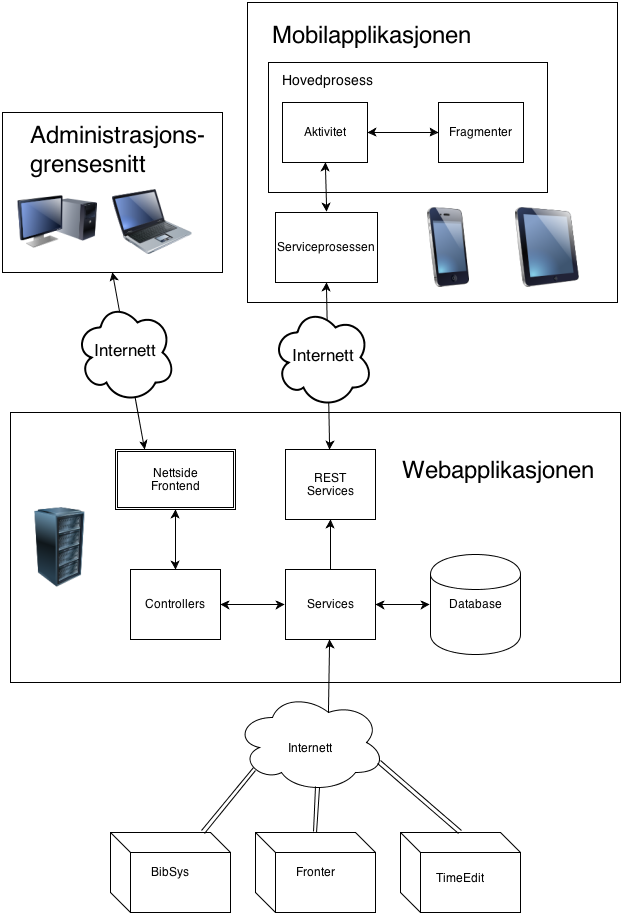
\includegraphics[width=9cm]{diagram.png}
  \caption{Oversikt over hele systemet}
\end{figure}

\section{Mobilapplikasjonen}

\begin{figure}[H]
        \centering
        \begin{subfigure}[b]{0.3\textwidth}
                \centering
                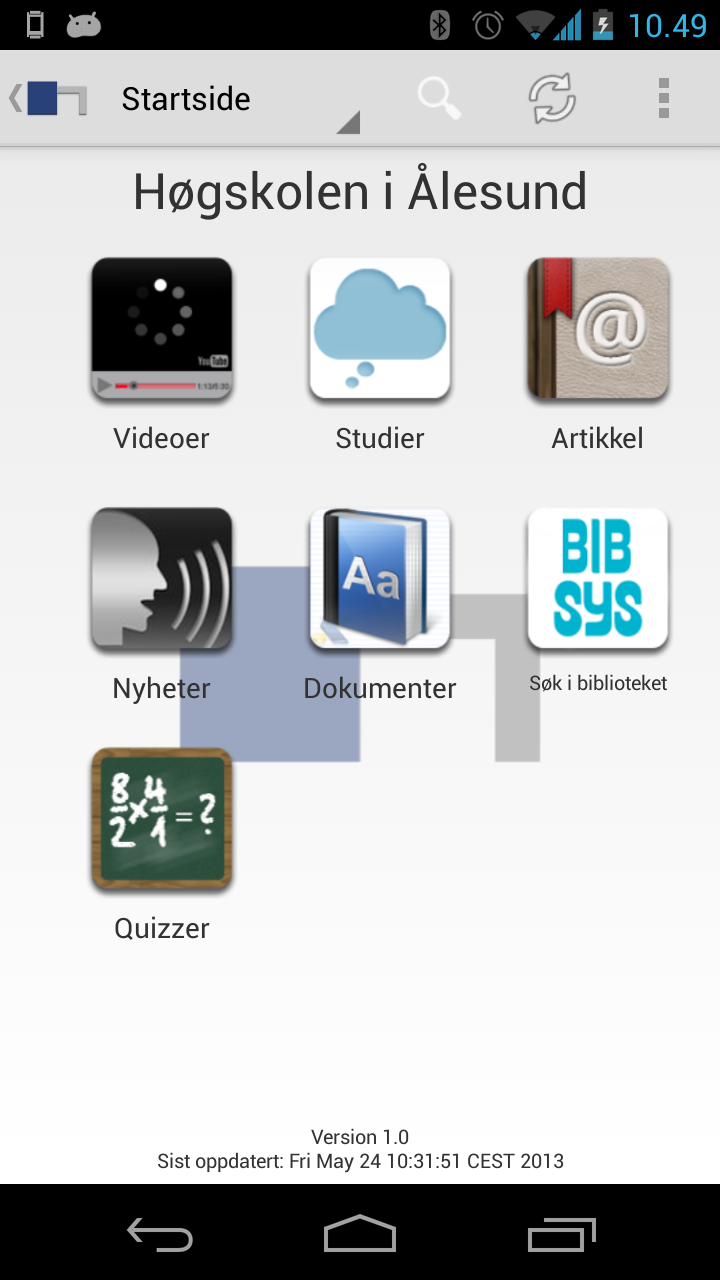
\includegraphics[width=5cm]{framside_mobil.png}
                \caption{På en mobiltelefon}
        \end{subfigure}
        \quad
        \begin{subfigure}[b]{0.3\textwidth}
                \centering
                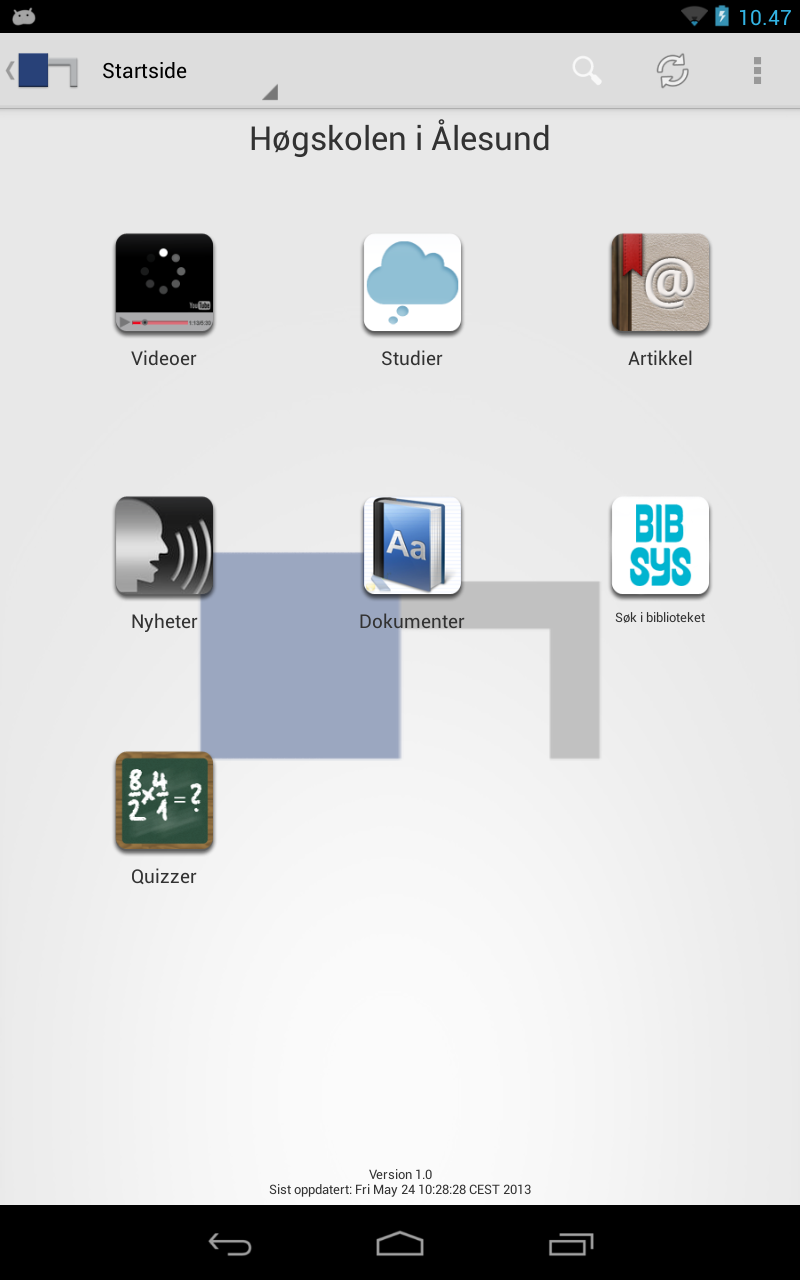
\includegraphics[width=6cm]{framside_nettbrett.png}
                \caption{På ett nettbrett}
        \end{subfigure}
        \caption{Skjermbilder av fremsiden til mobilapplikasjonen}
\end{figure}

Mobilapplikasjonene er laget for Android operativsystemet og bruker Android SDK versjon 14. Med unntak av slidingmeny funksjonen brukt i TimeEdit implementasjonen er all teknologien i applikasjonen inkludert i Android SDKet eller utviklet av prosjektmedlemmene. Med unntak av logoene til høgskolen, fronter og bibsys er ikonene til fragmentene hentet fra en åpen ikonpakke på nettet. Resten av grafikken er standard i Android SDKet.\newline
\newline
Endringer i mobilapplikasjonen fra forrige versjon (høsten 2012):
\begin{itemize}
\item Ikke lenger statiske fragmenter / data. I den forrige versjonen var alle fragmentene tilstede på alle sidene, selv om de ikke hadde innhold. Dette gjorde at alle lagen i applikasjonen så helt like ut og forvirret brukere.
\item Full omskriving av metodene for innlasting av data. Bruker nå kun et GET (se begreper) kall for å laste ned et studie/fag/etc. I forrige versjon var det en GET kall for hvert fragment/side. Dette gjorde at datainnlastingen tok lengre tid.
\item Full omskriving av JSON parsingen. I den tidligere versjonen var parsingen av objektene gjort i samme klasse som datainnlastingen. Nå har hver av dataklassene en konstruktør for JSON data og håndterer derfor parsingen selv. Dette har gjort det lettere å feilsøke parsingen og å legge til nye dataklasser.
\item Stabilitet. Bedre feilhåndtering og forenklet logikk har bidratt til å gjøre mobilapplikasjonen mye mer stabil.
\item Integrasjon av de eksterne tjenestene TimeEdit og BibSys. Mer om dette senere i rapporten.
\end{itemize}

\begin{figure}[H]
  \centering
  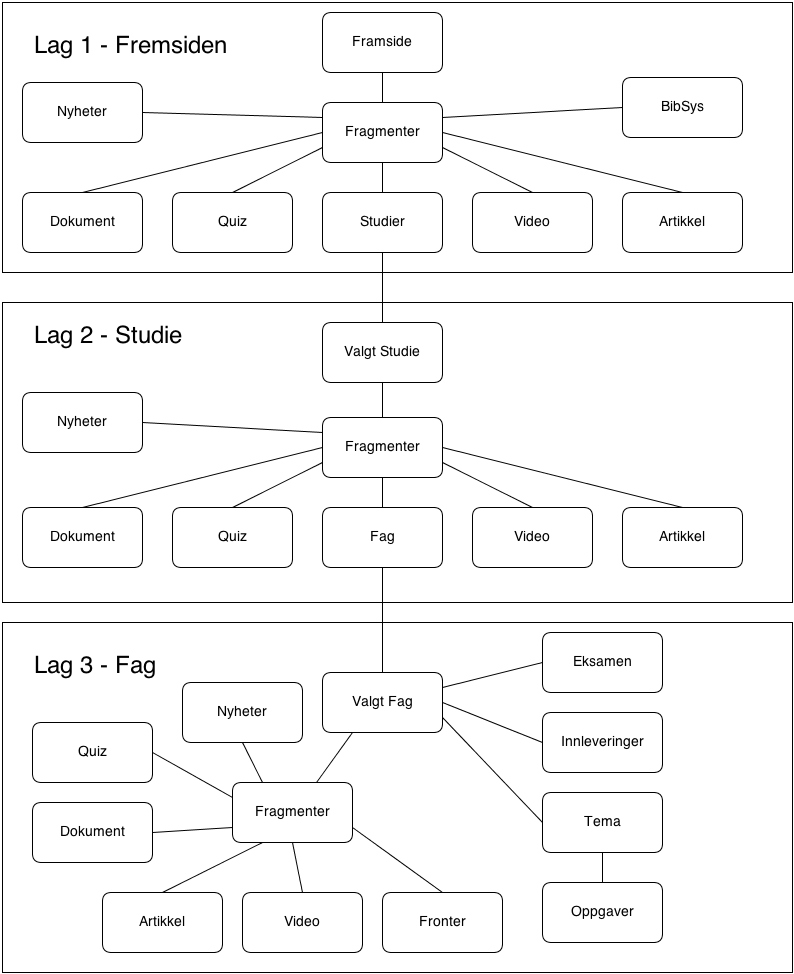
\includegraphics[width=9cm]{mobapp_modell.png}
  \caption{Viser objektene på hvert lag i mobilapplikasjonen og flyten mellom lagene}
\end{figure}

Mobilapplikasjonen er delt inn i tre lag. Lag 1 er fremsiden av applikasjonen og det første brukeren ser når applikasjonen startes. Her vises fragmentene som er knyttet til fremside objektet på webapplikasjonen som ikoner. På dette laget er det meningen å ha informasjon relatert til skolen i seg selv, for eksempel en spørreundersøkelses quiz eller nyheter om skolen. Når brukerene trykker på et av ikonene åpnes dette fragmentet og viser dets innhold. Får å komme tilbake til fragmentoversikten kan brukeren trykk på back knappen i android eller bruke rullegardin-menyen øverst i skjermbildet. Systemet kan bare ha en fremside.\newline
\newline
Når brukeren velger et studie fra studieliste-fragmentet går applikasjonen ned til neste lag. Lag 2 er studielaget, som på fremsiden vises fragmentene som er knyttet til studie i webapplikasjonen.\newline
\newline
Når brukeren velger et fag fra fagliste-fragmentet går applikasjonen videre til det siste laget. Lag 3 er faglaget, som de andre lagene inneholder dette laget fragmenter definert av webapplikasjonen. Fag-laget inneholder i tillegg ekstra datafelt for eksamener, innleveringer og tema med oppgaver.\newline
\newline
Grunnen til at denne strukturen ble valgt er at den ble spesifisert av kunden da systemet ble bestilt i 2012. Kravspesifikasjonen hvor strukturen ble beskrevet ble fremlagt og produsert av Harald Yndestad. Denne kravspesifikasjonen spesifiserte systemet som ble utviklet opp til starten av dette prosjektet.\newline

\subsection{Sammenligning med det gamle systemet}

\begin{figure}[H]
  \centering
  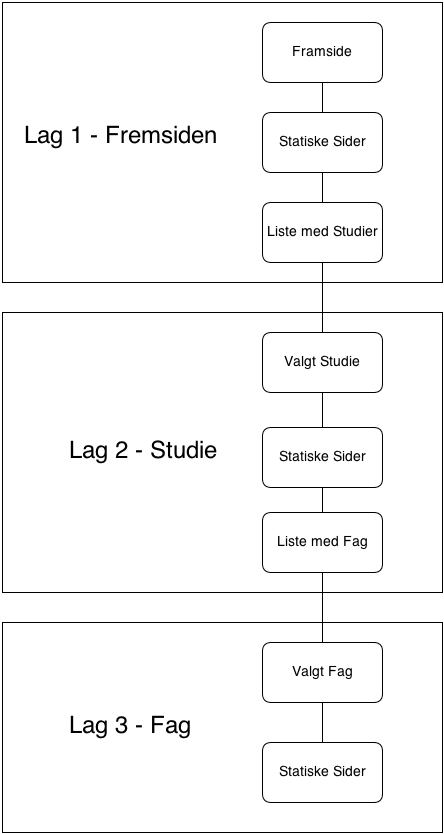
\includegraphics[width=7cm]{mobapp_modell_gammel.png}
  \caption{Viser flyten i det gamle systemet}
\end{figure}

I det gamle systemet hadde alle objektene på alle lagene de samme sidene. På fremsiden måtte ressurslinkene til informasjonen på serveren hardkodes inn i mobilapplikasjonen og kompileres hver gang det skulle gjøres en endring. Dette gjorde det gamle systemet veldig tungvint å vedlikeholde og gjorde systemet veldig sårbart mot systemkrasj om ressurser på serveren ble slettet. På lagene under (studier og fag) var informasjonen lagret som attributter i lag-objektet. Det vil si at hvert lag måtte ha en og bare en av hvert type dataobjekt (artikkel, videoer osv). Om lag-objektet manglet en ressurslink for et objekt eller linken til ressursen var ugyldig krasjet applikasjonen.

\subsection{Git statistikk}

Statistikk for endringer i mobilapplikasjonens github repository siden prosjektstart:
\begin{itemize}
\item Antall commits: 60
\item Antall linjer lagt til: 5513
\item Antall linjer slettet: 7474
\item Totalt antall linjer alle filer: 15308
\item Totalt antall linjer - Java kode: 8625
\item Totalt antall linjer - XML: 2146
\end{itemize}

\subsection{Installasjonsinstrukser}

For å installere mobilapplikasjonen på mobiltelefonen eller nettbrettet ditt trenger du minst versjon 4.0 (Ice Cream Sandwich) av Android operativsystemet. Siden applikasjonen ikke er tilgjengelig på Google Play butikken må den installeres manuelt, for å gjøre dette må du først tillate installering av eksterne applikasjoner gå inn på innstillinger -> sikkerhet og skru på “ukjente kilder”. Etter det er det bare å åpne den kompilerte .apk filen i prosjektmappen (Muldvarp/bin/Muldvarp-Debug.apk). Denne filen er også 
linket til på fremsiden av webapplikasjonen.

\subsection{Forklaring av brukergrensesnittet}

\begin{figure}[H]
  \centering
  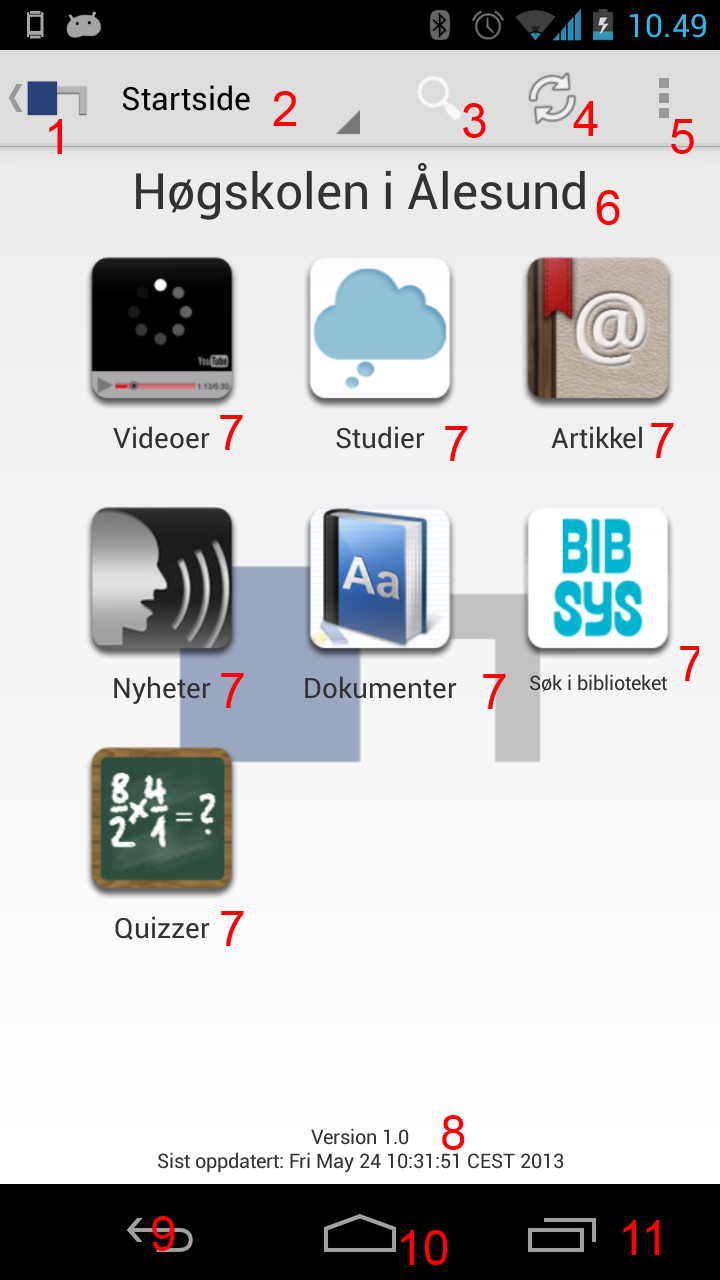
\includegraphics[width=4.5cm]{mobapp-ui-forklaring.png}
  \caption{Forklaring for brukergrensesnittet}
\end{figure}

\begin{enumerate}
\item Knapp for å få fram sidemenyen. Sidemenyen inneholder timeplan funksjonen.
\item Tittelen på fragmentetsiden du er på nå. Trykk her for å få opp en rullegardin-meny der du kan navigere til de andre fragmentene i laget.
\item Søkeknapp. Trykk her når du er i en liste for å filtrere listen med søkeordet ditt.
\item Oppdateringsknapp / “Refresh”. Oppdaterer og laster ned informasjonen om siden du er på nå på nytt.
\item Diverse. Her finner du innloggingsknappen (ikke ferdig implementert) og en “om oss” knapp som popper opp et vindu med diverse informasjon om høgskolen som for eksempel postaddresse.
\item Tittelen på laget du befinner deg på. I dette tilfellet fremsiden. Når du er på studie eller fag nivået vises navnet til studiet / faget.
\item Fragmentene på laget. Trykk på ett fragment for å navigere til den siden.
\item Informasjon om applikasjonsversjonen og når dataen for laget du befinner deg på sist ble lastet inn.
\item Tilbake-knapp. Standard i Android operativsystemet. Trykk her når du er på fragmentoversikten for å bevege deg opp et lag, trykk på knappen når du befinner deg i en fragmentside for å gå tilbake til fragmentoversikten.
\item Hjem-knapp. Standard i Android operativsystemet. Trykk her for å ut av applikasjonen. Applikasjonen lukkes ikke men legges i bakgrunnen.
\item Applikasjonsvelger-knapp. Standard i Android operativsystemet. Trykk her for å velge applikasjoner som kjører i bakgrunnen.
\end{enumerate}

\subsection{Serviceprossesen}

Serviceprossesen er en egen prosses som kjører parallelt med applikasjonens hovedprosses. Den har ansvar for å hente data fra serveren, parse dataen og lagre dataobjektene i minne

\subsection{Datainnlasting}

Mobilapplikasjonen laster inn data fra webapplikasjonen via REST tjenestene på serveren. Tjenestene leverer dataen i JSON format som blir parset og lagret i minnet av serviceprosessen.

\begin{figure}[H]
  \centering
  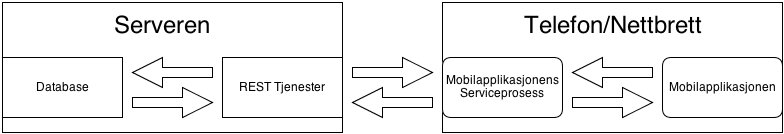
\includegraphics[width=12cm]{flytdiagram-data.png}
  \caption{Viser flyten mellom webapplikasjonen og mobilapplikasjonen}
\end{figure}

Først lager hovedprosessen en tilkobling til serviceprosessen og sender en førespørsel om dataen den trenger. Så laster serviceprosessen ned og parser dataene hovedprosessen forespurte. Når informasjon er ferdig parset av serviceprosessen, sender den en melding til hovedprosessen om at informasjon er klar til bruk. Deretter henter hovedprosessen informasjonen fra serviceprosessen og gjør den tilgjengelig for bruk av fragmentene.\newline
For eksempel så vil første innlasting av data til mobilapplikasjonen bestå av kall til “frontpage” for å få fragmentene til fremsiden, “programme” for å hente en liste av alle studiene, “articles/news” for å få nyhetene og “timeedit/<klasseid>” for å hente brukerens timeplan. Senere vil mobilapplikasjonen sende førespørsler etter mer data etter behov. Se seksjonen om webapplikasjonen i resultatdelen for nærmere oversikt over de forskjellige tjeneste-kallene

\subsection{Fragmenter/Moduler}

Mobilapplikasjonen er bygd opp av flere lag der hvert lag har flere fragmenter (se begreper) eller sider med forskjellig informasjon. Disse fragmentene styres av laget (aktiviteten, se begreper) som henter frem og viser fragmenter etter behov. Hvilke fragmenter som er på hvilket lag og objekt er definert av webapplikasjonen. Her er en oversikt over de forskjellige typene fragmenter.

\subsubsection{Lister}

Store deler av applikasjonens sider består av lister over andre objekter. Disse listene kan inneholde alle de forskjellige dataobjekt typene. I disse listene kan brukerene filtrere listen med et søkeord med forstørrelsesglass knappen i toppmenyen


\subsubsection{Artikkel / Nyheter}

\begin{figure}[H]
        \centering
        \begin{subfigure}[b]{0.3\textwidth}
                \centering
                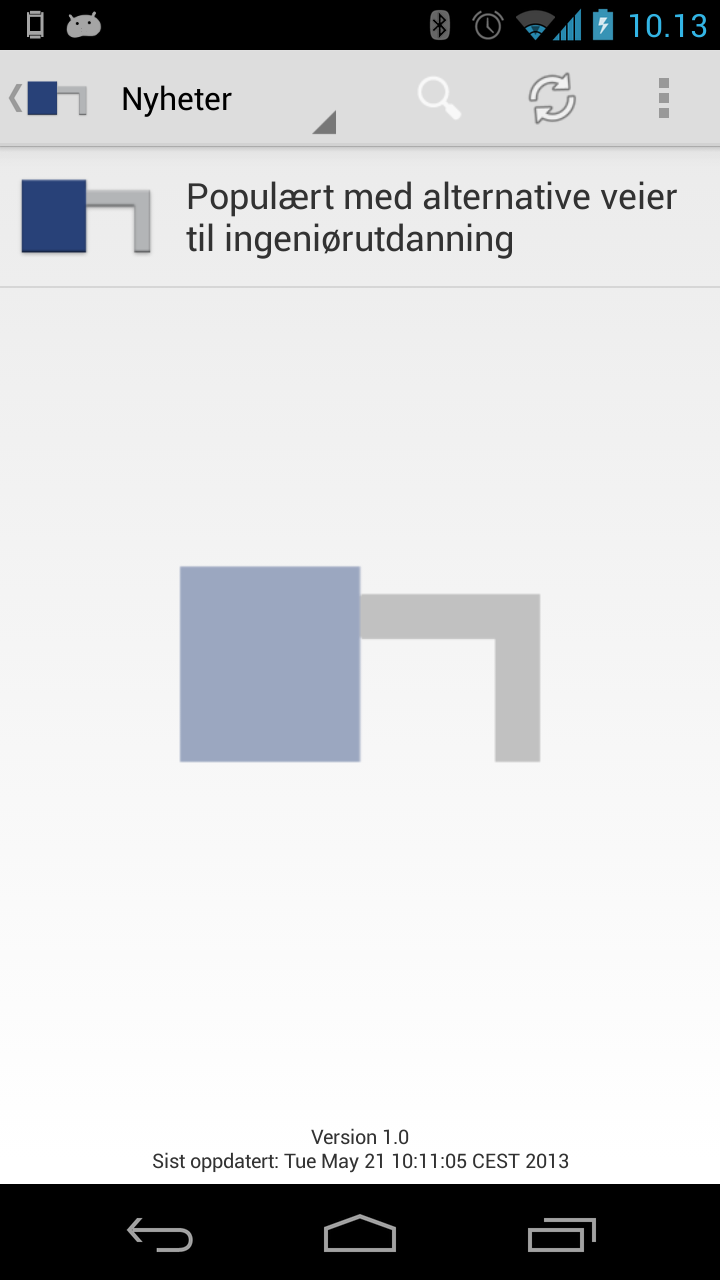
\includegraphics[width=5cm]{artikkel1.png}
                \caption{Liste med nyheter}
        \end{subfigure}
        \quad
        \begin{subfigure}[b]{0.3\textwidth}
                \centering
                
\includegraphics[width=5cm]{artikkel2.png}
                \caption{En artikkel}
        \end{subfigure}
        \caption{Skjermbilder av artikkel-funksjonen til mobilapplikasjonen}
\end{figure}

Artikkel fragmentet viser en HTML side fra webapplikasjonen i et standard WebView i Android. Nyhetsfragmentet viser en liste med artikler fra valgt kategori, når du velger en får du samme visning som artikkel fragmentet.

\subsubsection{Studier / Fag}

\begin{figure}[H]
        \centering
        \begin{subfigure}[b]{0.3\textwidth}
                \centering
                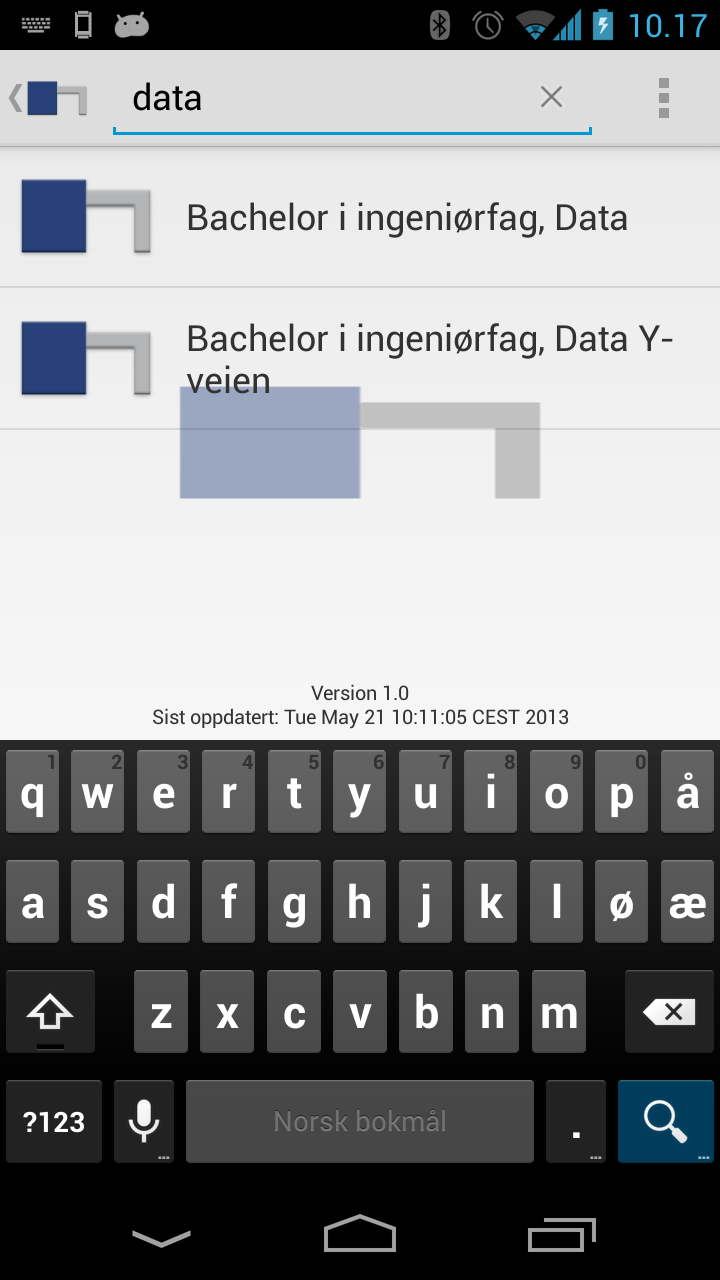
\includegraphics[width=5cm]{studier1.png}
                \caption{En liste med studier filtrert med søkeordet "data"}
        \end{subfigure}
        \quad
        \begin{subfigure}[b]{0.3\textwidth}
                \centering
                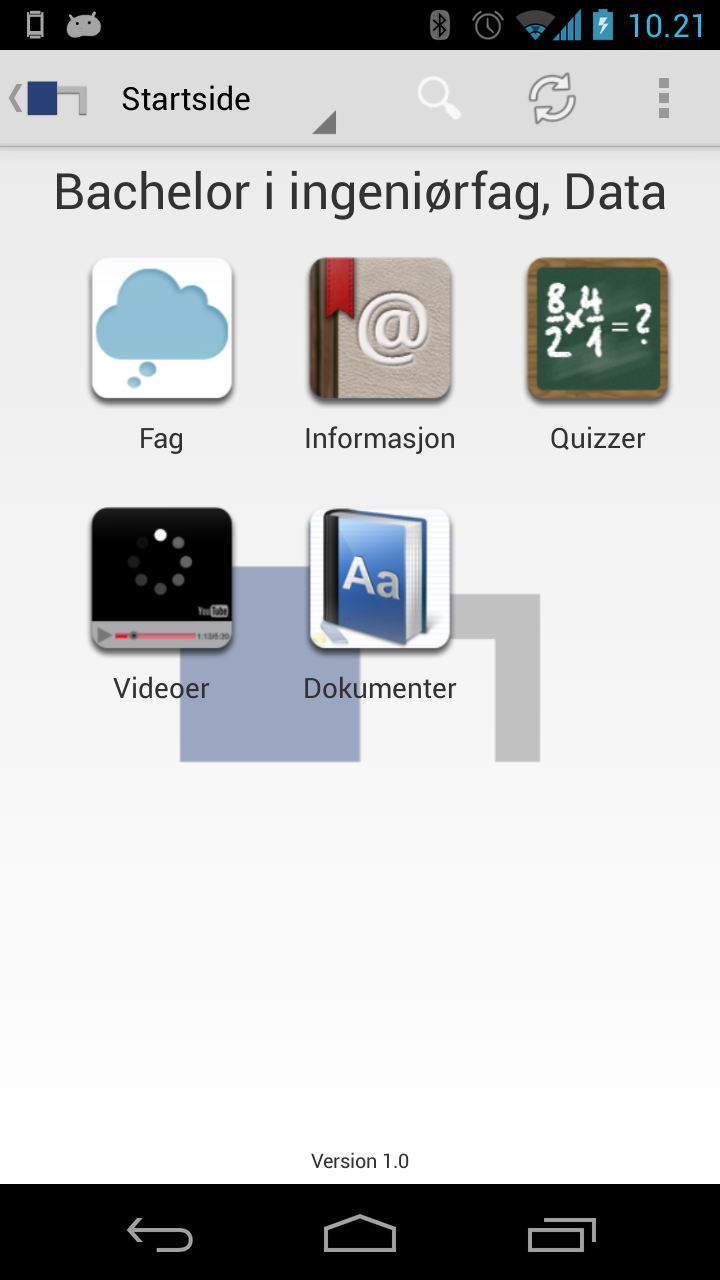
\includegraphics[width=5cm]{studier2.png}
                \caption{Startsiden til studie-laget}
        \end{subfigure}
        \caption{Skjermbilder av studie/fag-funksjonen til mobilapplikasjonen}
\end{figure}

Viser en liste over alle studier / fag i valgte studie. Når du velger et studie eller fag går du “ned et lag” til det valgte studie / faget. Her vises studielisten filtrert med søkeordet “data” og fremsiden til det valgte objektet i studielaget.

\subsubsection{Dokumenter}

\begin{figure}[H]
        \centering
        \begin{subfigure}[b]{0.3\textwidth}
                \centering
                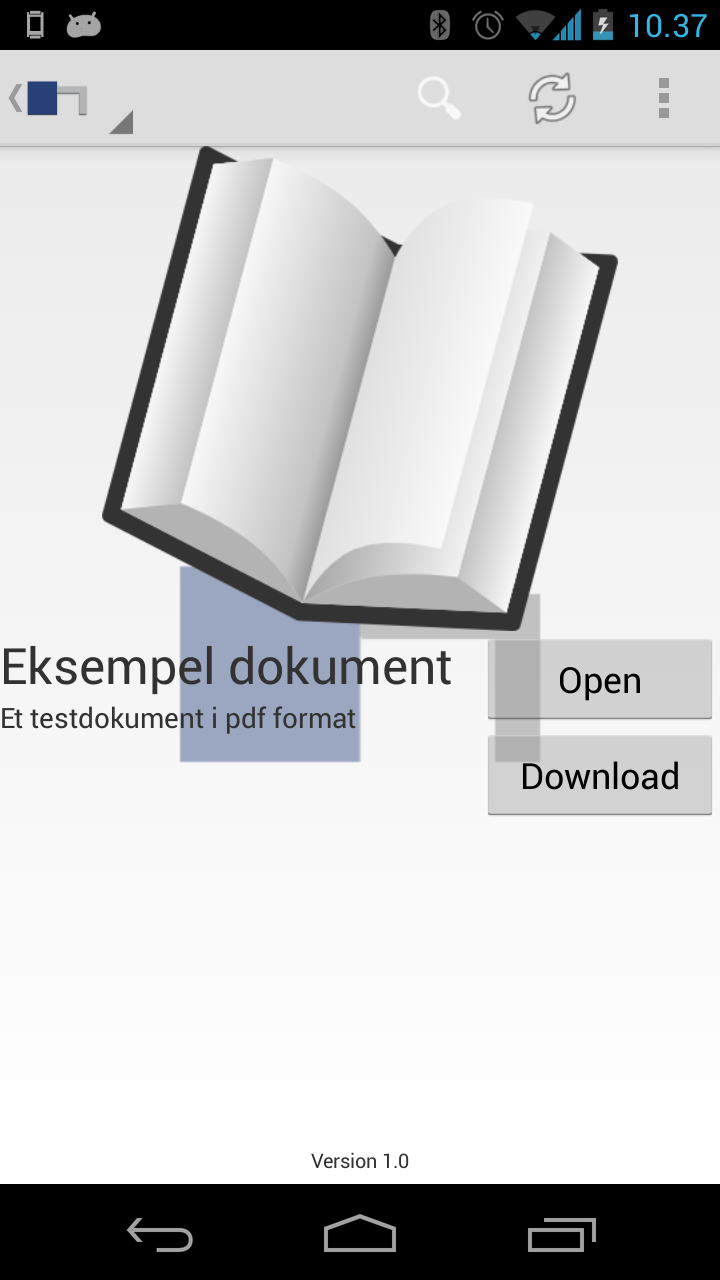
\includegraphics[width=5cm]{dokumenter1.png}
                \caption{Detaljesiden til et dokument}
        \end{subfigure}
        \quad
        \begin{subfigure}[b]{0.3\textwidth}
                \centering
                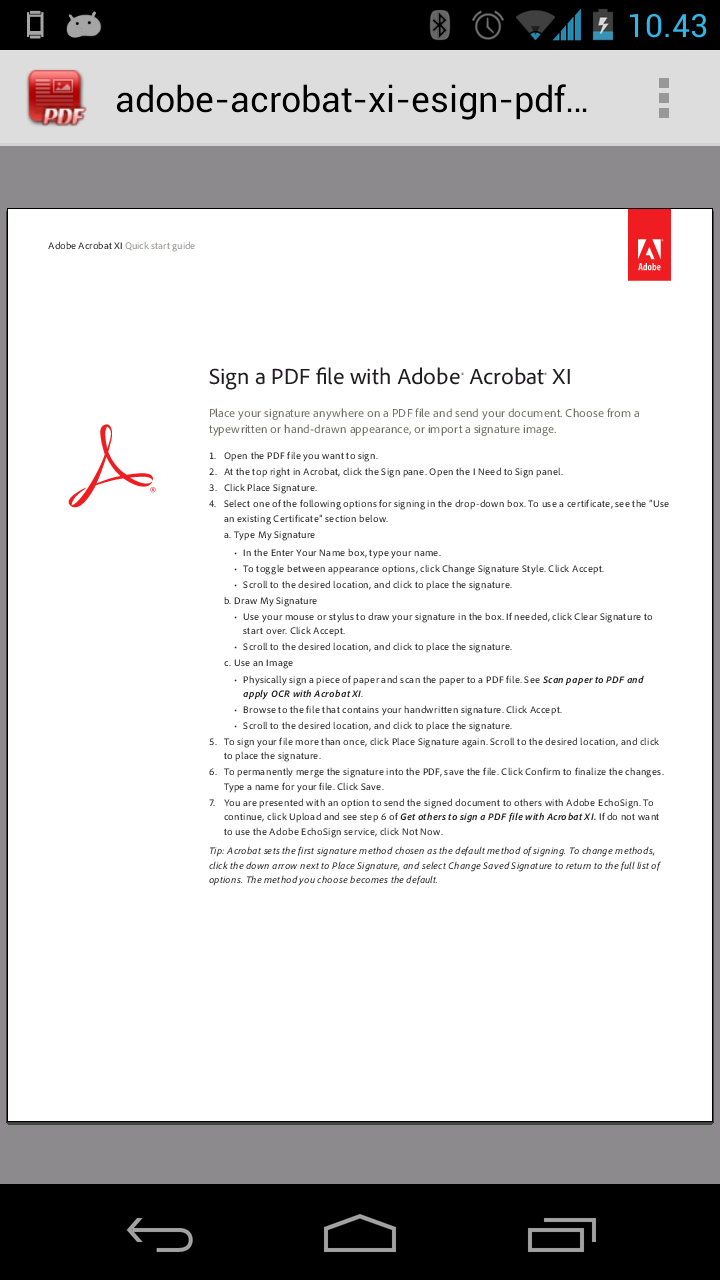
\includegraphics[width=5cm]{dokumenter2.png}
                \caption{Et dokument}
        \end{subfigure}
        \caption{Skjermbilder av dokument-funksjonen til mobilapplikasjonen}
\end{figure}

Inneholder en liste over alle dokumentene knyttet til fragmentet. Når klikker på et dokument i listen får du opp en oversiktsside med informasjon om det valgte dokumentet. Trykk på “Open” for å åpne dokumentet i mobilen/nettbrettets standard dokumentvisnings-applikasjon. Trykk “Download” for å laste ned filen til mobilen/nettbrettes standard nettlastingsmappe

\subsubsection{Video}

\begin{figure}[H]
        \centering
        \begin{subfigure}[b]{0.3\textwidth}
                \centering
                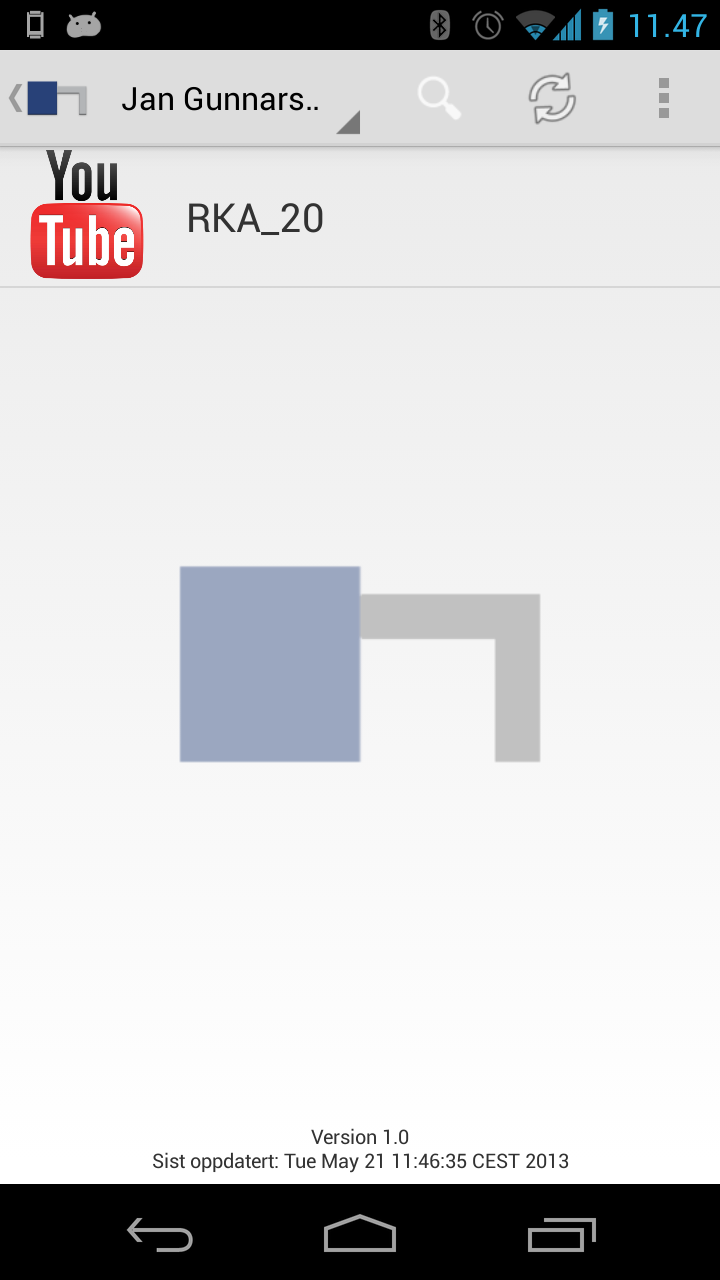
\includegraphics[width=5cm]{video1.png}
                \caption{Videoliste}
        \end{subfigure}
        \quad
        \begin{subfigure}[b]{0.3\textwidth}
                \centering
                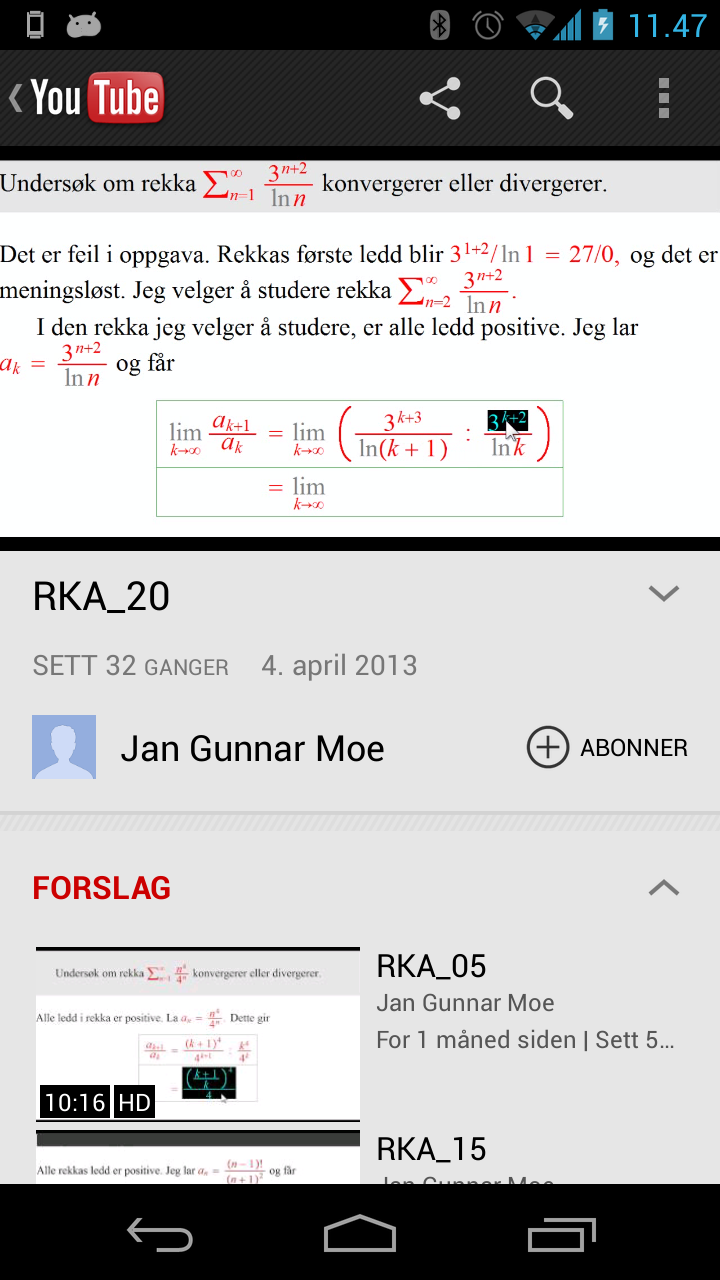
\includegraphics[width=5cm]{video2.png}
                \caption{Åpnet YouTube-video}
        \end{subfigure}
        \caption{Skjermbilder av video-funksjonen til mobilapplikasjonen}
\end{figure}

Video fragmentet inneholder en liste av alle videoer knyttet til fragmentet. Når du velger en video åpner videoprogrammet på mobilen, i dette tilfellet YouTube

\subsubsection{Quiz}

Quiz-seksjonen av mobil-applikasjonen tilbyr quizzer eller andre type spørringer til brukerene. Av de forskjellige typene er kun de som ikke kommuniserer svar tilbake til server implementert grunnet mangel av sentralt brukersystem.
Quiz-fragmentet som tilgjengelig fra hovedsiden inneholder en liste over quizzer som er knyttet til hovedsiden’s lagtype - fag, kurs eller genere

\begin{figure}[H]
        \centering
        \begin{subfigure}[b]{0.3\textwidth}
                \centering
                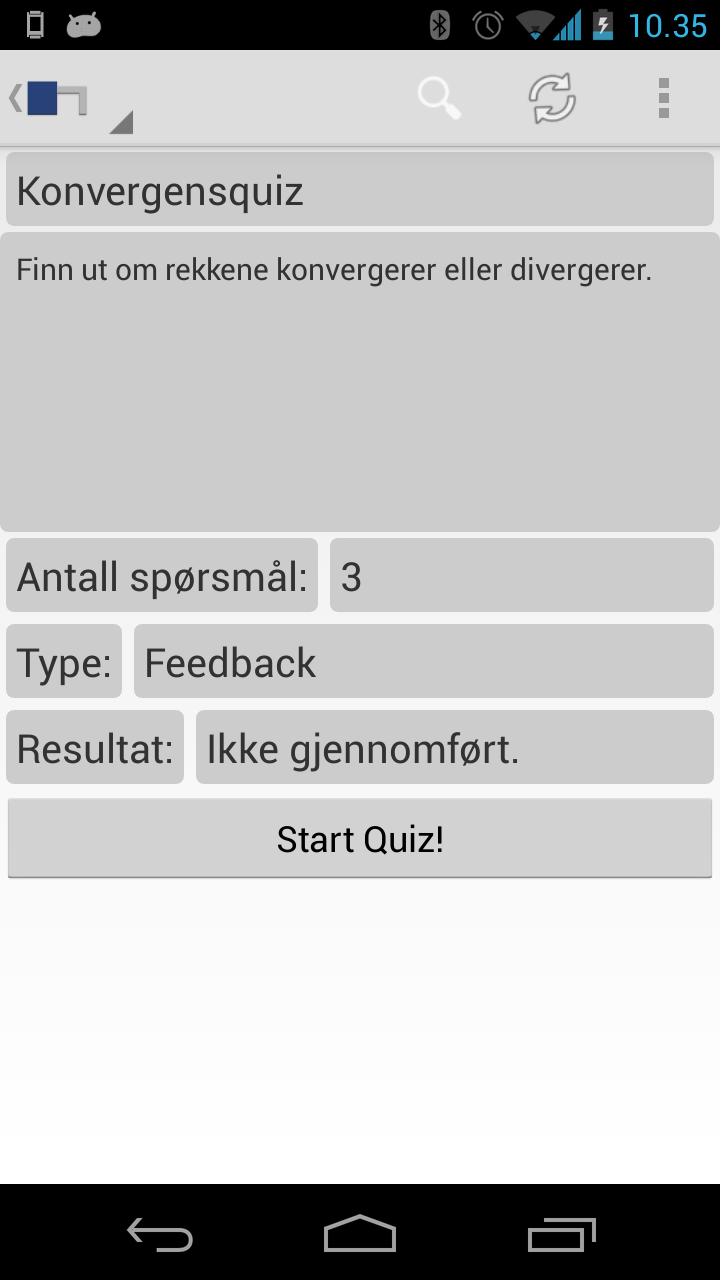
\includegraphics[width=5cm]{quiz1.png}
                \caption{Startsiden til en quiz}
        \end{subfigure}
        \quad
        \begin{subfigure}[b]{0.3\textwidth}
                \centering
                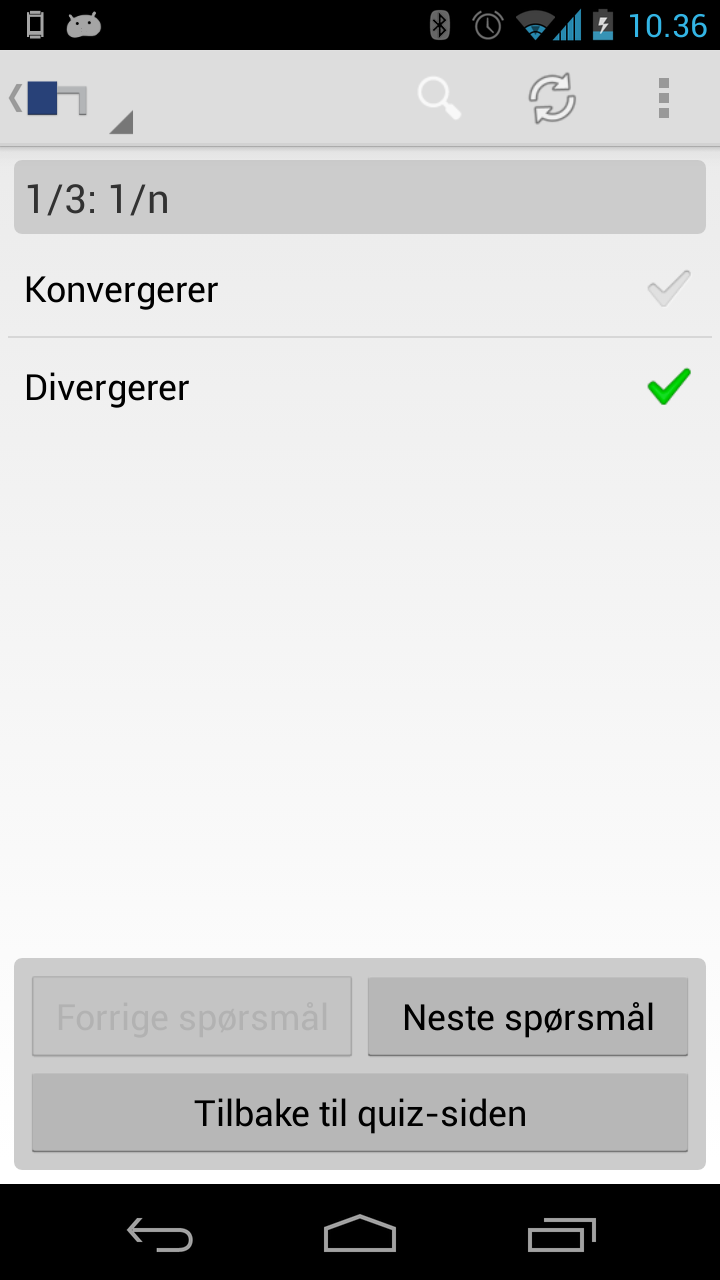
\includegraphics[width=5cm]{quiz2.png}
                \caption{Et dokument}
        \end{subfigure}
        \caption{Skjermbilder av quiz-funksjonen til mobilapplikasjonen}
\end{figure}

Etter å ha valgt en quiz får du opp startskjermen med informasjon om quizzen. Her står det en kort beskrivelse av innholdet, og antall spørsmål quizzen inneholder. Quizzen startes herfra ved å trykke på “Start Quiz!”.
Oppgavene eller spørsmålene kan være flervalgs eller enkeltvalgs-typer, og advarsler vil komme opp dersom ingen alternativ er valgt. Navigasjon mellom alle spørsmålene er også mulig, og ved siste vil man å en advarsel om at er i ferd med å avslutte Quizzen og gå til resultatskjermen. Man er også i stand til å avslutte Quizzen når som helst, og dette vil forkaste alle svar.

\begin{figure}[H]
        \centering
        \begin{subfigure}[b]{0.3\textwidth}
                \centering
                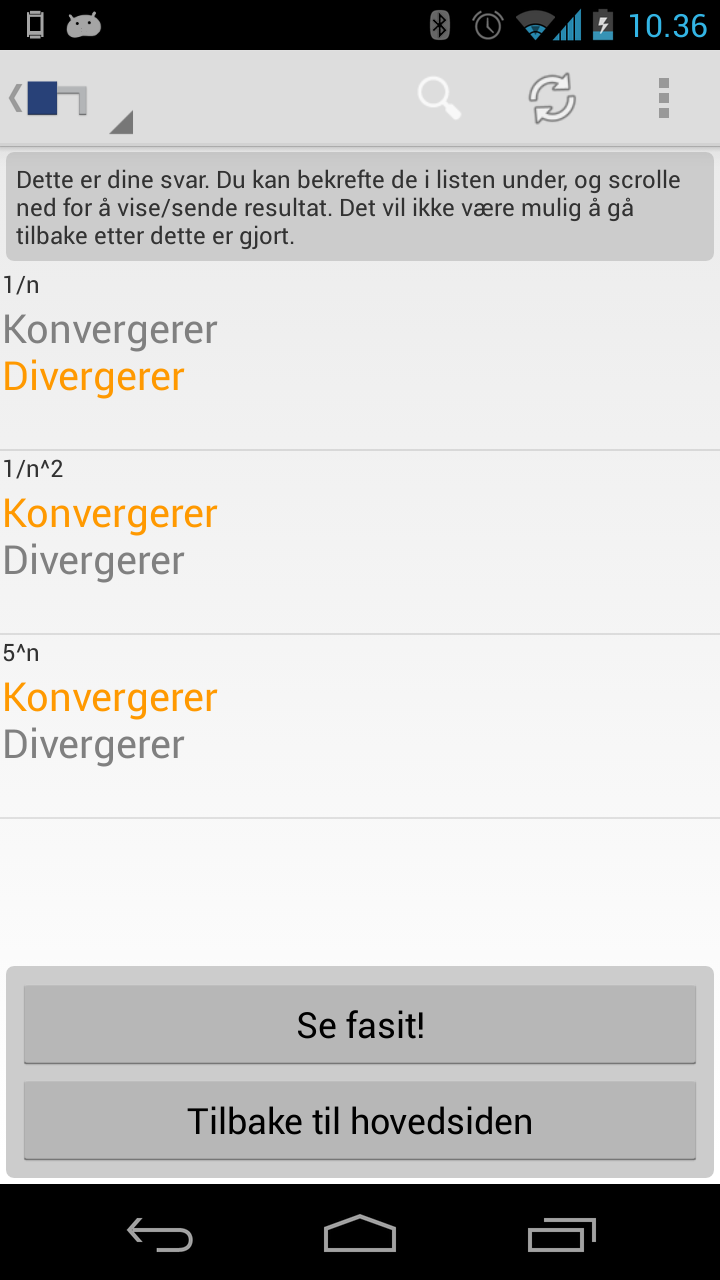
\includegraphics[width=4cm]{quiz3.png}
                \caption{Viser dine svar}
        \end{subfigure}
        \quad
        \begin{subfigure}[b]{0.3\textwidth}
                \centering
                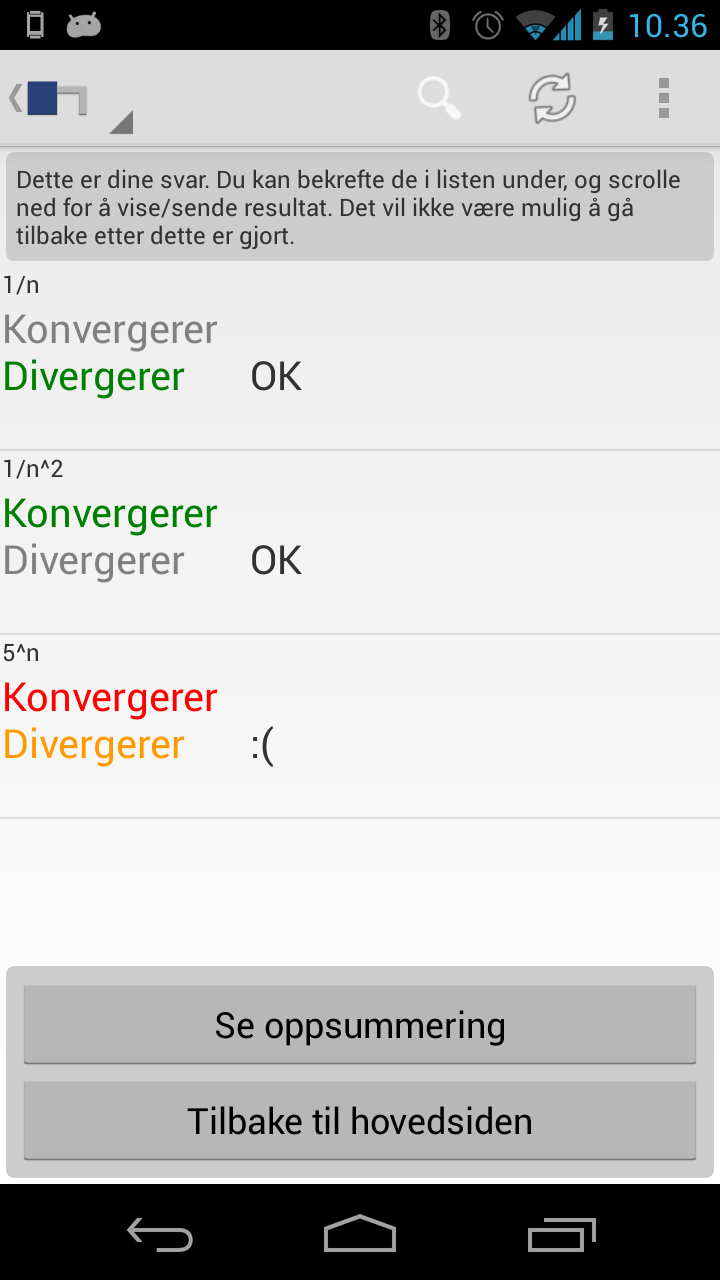
\includegraphics[width=4cm]{quiz4.png}
                \caption{Viser korrekte svar}
        \end{subfigure}
        \quad
                \begin{subfigure}[b]{0.3\textwidth}
                        \centering
                        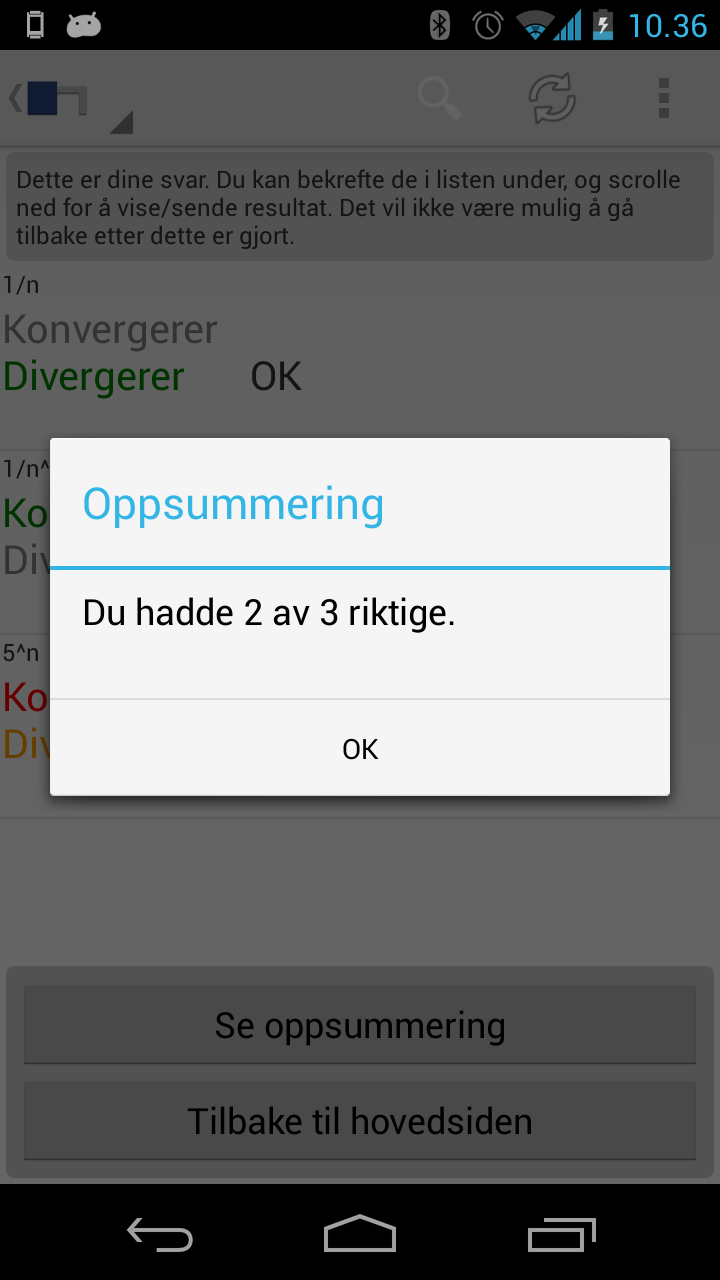
\includegraphics[width=4cm]{quiz5.png}
                        \caption{Oppsummering}
                \end{subfigure}
        \caption{Skjermbilder av quiz-funksjonen til mobilapplikasjonen}
\end{figure}

Etter man har svart på alle spørsmålene kommer man til en oppsummeringsside. Her vises ett sammendrag av alle spørsmålene og hvilke alternativer som ble valgt. Ved å trykke på “se fasit” knappen nederst på siden får man opp de riktige alternativene, som viser hvilke svar du har valgt og om de er riktige eller gale. Kjent fargekoding forklarer visuelt gale/riktige svar.
Videre kan man trykke oppsummeringsknappen for å se en opptelling riktige svar mot hvor mange som var mulig å få riktig, og eventuelt en vurdering






\section{Webapplikasjonen}

\begin{figure}[H]
  \centering
  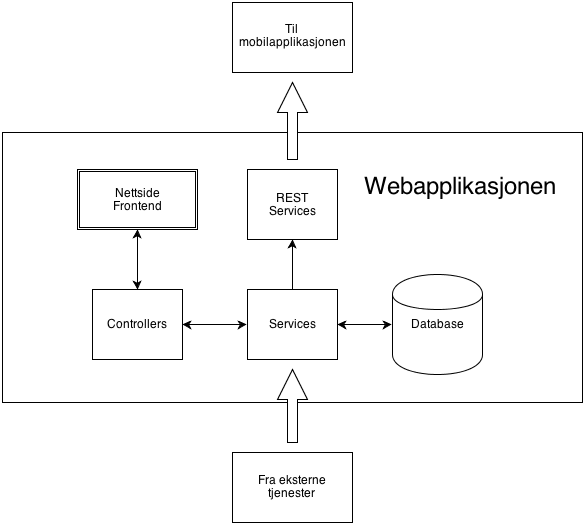
\includegraphics[width=9cm]{webapp_modell.png}
  \caption{Oversikt over webapplikasjonen}
\end{figure}

Webapplikasjonen er laget på Java Enterprise Edition 6 plattformen. Arkitekturen er basert på Model View Controller-modellen, men avviker noe fra modellen (mer om dette senere i rapporten). Webapplikasjonen har en nettsidefrontend for administrasjon og et sett med REST tjenester for å gjøre dataen lett tilgjengelig for eksterne applikasjoner som mobilapplikasjonen. I dette prosjektet publiserte vi webapplikasjonen på en GlassFish Open Source Edition server, men den kan også publiseres på andre webapplikasjonsservere som støtter Java Enterprise Edition 6 webapplikasjoner. \newline
\newline
Teknologier brukt i webapplikasjonen:
\begin{itemize}
\item Java Enterprise Beans - Plattformen webapplikasjonen er utviklet på.
\item JavaServer Faces - Brukt til frontenden/nettsiden.
\item PrimeFaces - Komponentbibliotek til JavaServer Faces. Brukt til redigeringssidene og navigasjonssystemet i frontenden.
\item JSoup - Brukt til parsing av HTML og XML i TimeEdit og BibSys implementasjon
\item REST - Brukt til å eksponere data (API) til mobilapplikasjonen
\item JSON - Brukt som dataformat i REST tjenestene
\end{itemize}
For mer informasjon om teknologiene, se teoretisk grunnlag.\newline
\newline
Endringer i webapplikasjonen siden forrige versjon (høsten 2012)
\begin{itemize}
\item Dynamisk fragment system. Nå defineres fragmentene på mobilapplikasjonssiden i webapplikasjonen. Dette står for den største delen av oppgraderingen i den nye versjonen.
\item Stabilitet og feilfiksing. Den forrige versjonen var full av krasjbugs og feil i relasjonsdatabasen. Mye arbeid ble gjort for å finne og fikse feilene. For mer informasjon om relasjonsdatabasefeilene se seksjonen om drøfting.
\item Grafisk oppussing. Laget ny template og css stil. Samkjørt grafikken med mobilapplikasjonen. Laget ny fremside, med presentasjon av applikasjonens funksjoner og nedlastingslink til mobilapplikasjonen.
\item Skrevet om redigeringssidene. Redigeringssidene for lagobjektene er helt skrevet om for å bruke det nye fragmentsystemet.
Laget dokumentasjonsider.
\end{itemize}

\subsection{Git statistikk}

Statistikk for endringer i webapplikasjonens github repository siden prosjektstart:
\begin{itemize}
\item Antall commits: 101
\item Antall linjer lagt til: 15504
\item Antall linjer slettet: 9963
\item Totalt antall linjer 30336
\item Totalt antall linjer Java-kode: 8167
\item Totalt antall linjer xhtml / jsf: 7090
\end{itemize}

\subsection{Installasjonsinstrukser}

Webapplikasjonen kompileres til en .war fil. Denne filen kan publiseres på flere typer webapplikasjonsservere. I vårt prosjekt brukte vi GlassFish Open Source Edition som vår webapplikasjonsplattform, derfor er disse instruksjonene kun for GlassFish.

\subsubsection{Sette opp databasen:}

\begin{enumerate}
\item Trykk på “Resources” i venstremenyen
\item Trykk på “JDBC Connection Pools”
\item Trykk “New”
\item I feltet “Pool Name” skriv “MuldvarpPool”
\item Under “Resource Type” velg “javax.sql.DataSource”
\item Under “Database Driver Vendor” velg “JavaDB”
\item Trykk “Next”
\item Under “Additional Properties” i bunnen av siden fyll inn feltene som vist på bildet
\item Trykk “Finish
\end{enumerate}

\begin{figure}[H]
  \centering
  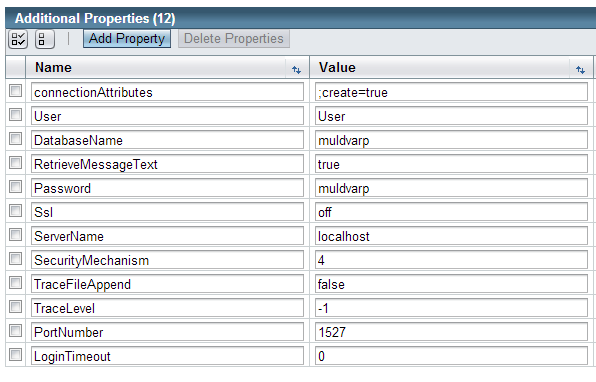
\includegraphics[width=12cm]{glassfish_jdbc.png}
  \caption{JDBC innstillinger}
\end{figure}

\begin{enumerate}
\setcounter{enumi}{9}
\item Gå til “JDBC Resources” i venstremenyen
\item Trykk “New”
\item I feltet “JNDI Name” skriv “jdbc/muldvarp”
\item Under “Pool Name” velg “MuldvarpPool”
\item Trykk “OK”
\end{enumerate}

\subsubsection{Sette opp administratorbruker}

\begin{wrapfigure}{l}{3.5cm}
  \begin{center}
    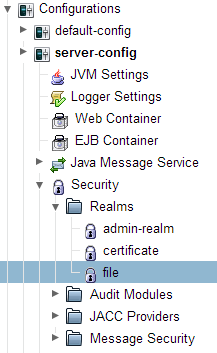
\includegraphics[width=3.5cm]{glassfish_filerealm.png}
  \end{center}
  \caption{Viser hvor file realm er}
\end{wrapfigure}

Webapplikasjonen bruker også “security-constraint” funksjonen i Java EE for å begrense tilgang til sidene i /admin/ mappen. \newline
\newline
For å konfigurere administratorbrukeren:
\begin{enumerate}
\item Trykk på “server-config” under “Configurations” i venstremenyen
\item Under “Security” velg “Realms” og så “file”
\item Skriv inn “Admin” i feltet “Assign Groups”
\item Trykk “Save”
\item Trykk på “Manage Users”
\item Trykk “New” for å legge til en ny bruker
\item Skriv “Admin” i feltene “User ID” og “Group List”
\item Skriv inn valgfritt passord
\item Trykk “Save”
\end{enumerate}

\subsubsection{Publiser applikasjonen}
\begin{enumerate}
\item Gå til “Applications” i venstremenyen
\item Trykk “Deploy”
\item Under “Packaged File to Be Uploaded to the Server” trykk “velg fil” og velg .war filen (MuldvarpWeb/target/MuldvarpWeb-1.1-TEST.war)
\item Under “Context Root” skriv “hials” (Dette blir adressen til webapplikasjonen)
\item Om applikasjonen allerede er publisert kryss av på “Force Redeploy” for å overskrive den
\item Trykk “OK”
\end{enumerate}

Applikasjonen er nå klar til bruk og kan nås med adressen “http://domene.no/hials”. Om glassfish ikke kjører på port 80 må du legge til portnummeret i adressen (eg. http://domene.no:8080/hials).

\subsubsection{Sett webapplikasjonen til standardapplikasjon}

For at webapplikasjonen skal visest i rot-adressen (eg. eapp.uials.no) må du gjøre følgende steg for å sette webapplikasjonen som standardapplikasjon

\begin{enumerate}
\item Trykk på “server-config” under “Configurations” i venstremenyen
\item Trykk på “Virtual Servers”
\item Trykk på “server”
\item Under “Default Web Module” velg “MuldvarpWeb-1.1-TEST”
\item Trykk “Save”
\end{enumerate}
Nå er webapplikasjonen tilgjengelig på rot-adressen til serveren.

\subsection{Administrasjonsgrensesnitt}

Administrasjonsgrensesnittet er utviklet i JavaServer Faces og bruker spesielt funksjoner og komponenter fra Primefaces biblioteket. Grensesnittet er delt inn i flere faner, en fane for hvert type objekt i systemet

\subsubsection{Fremside}

\begin{figure}[H]
  \centering
  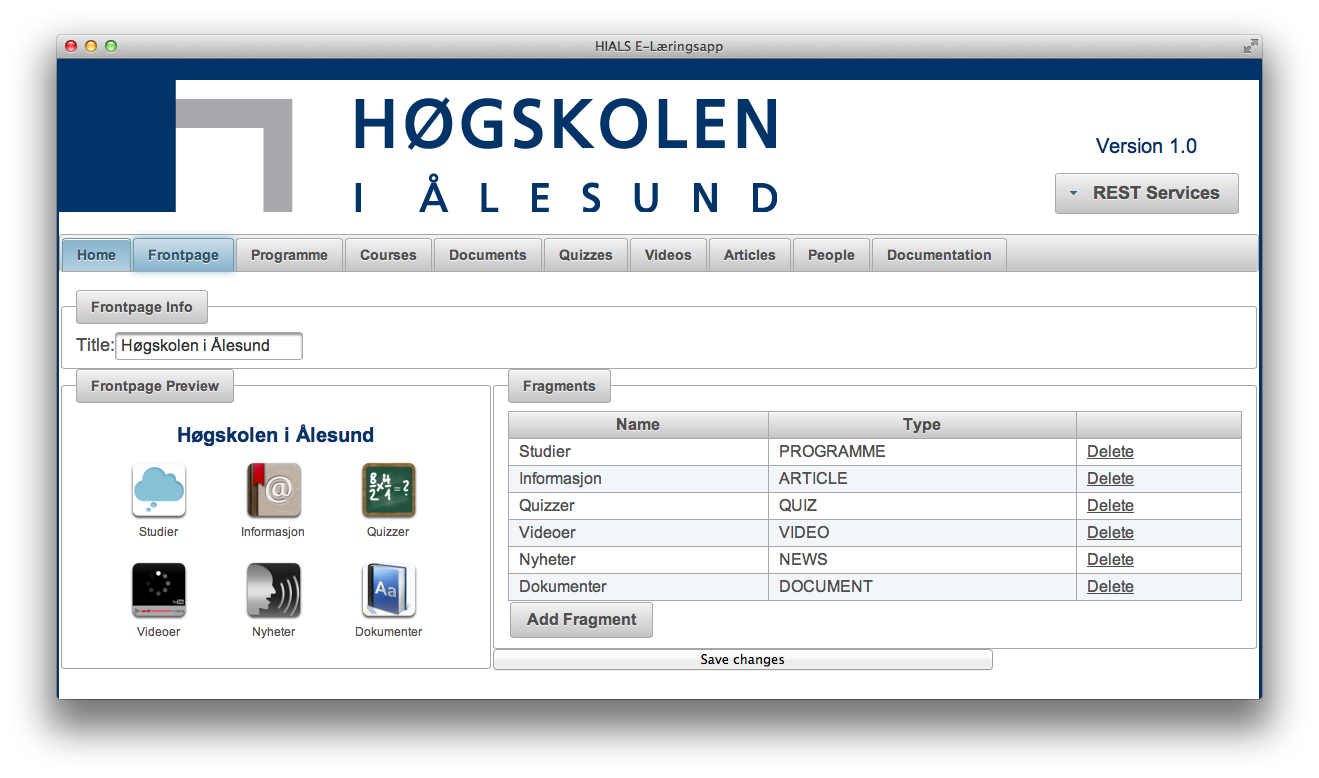
\includegraphics[width=12cm]{webapp_frontpage.png}
  \caption{Skjermbilde av webapplikasjonen - Viser framside-redigeringssiden}
\end{figure}

Her kan tittelen og hvilke fragmenter som skal vises på fremsiden av mobilapplikasjonen styres. Her får også administratoren en forhåndsvisning av hvordan dette vil se ut på mobilapplikasjonen.

\subsubsection{Studier}

\begin{figure}[H]
  \centering
  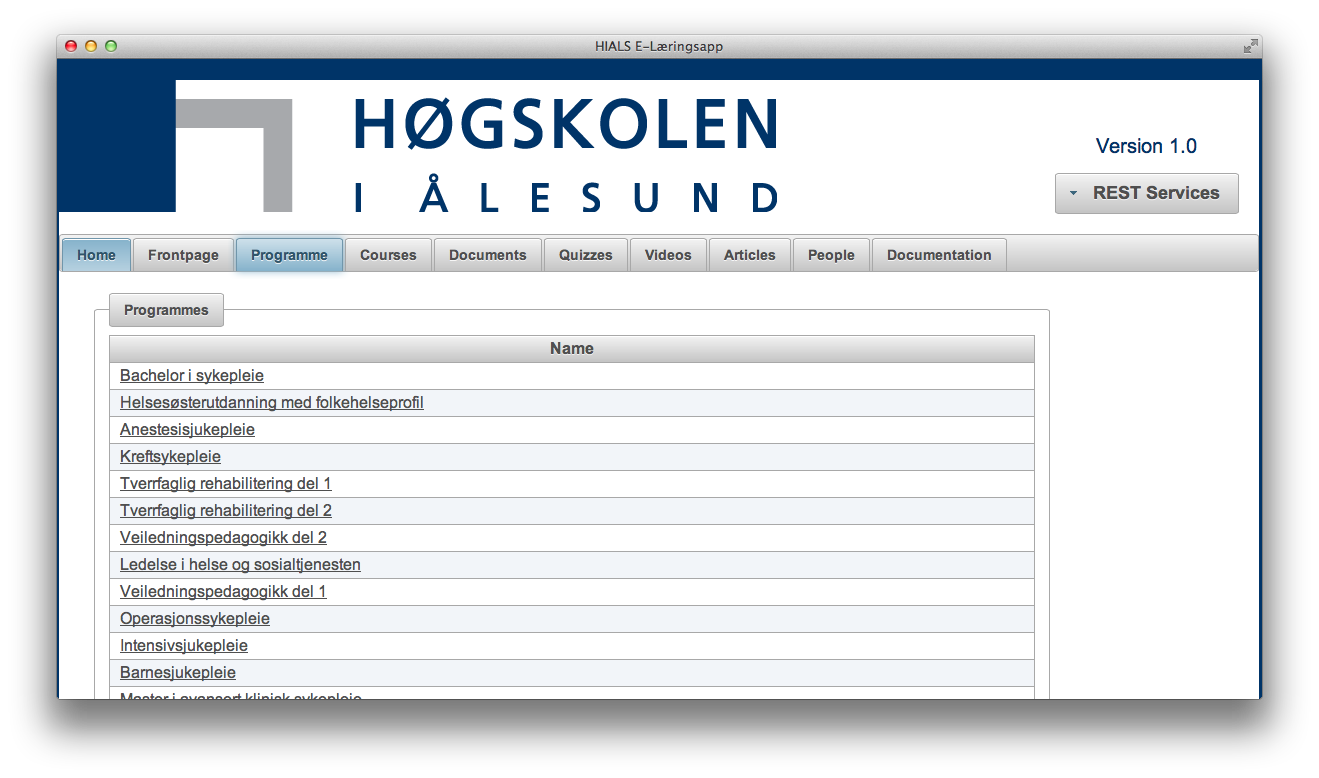
\includegraphics[width=12cm]{webapp_studieliste.png}
  \caption{Skjermbilde av webapplikasjonen - Viser listen over studier}
\end{figure}

Her vises en liste over alle studier i systemet. Her kan nye studier opprettes og eksisterende studier redigeres.

\begin{figure}[H]
  \centering
  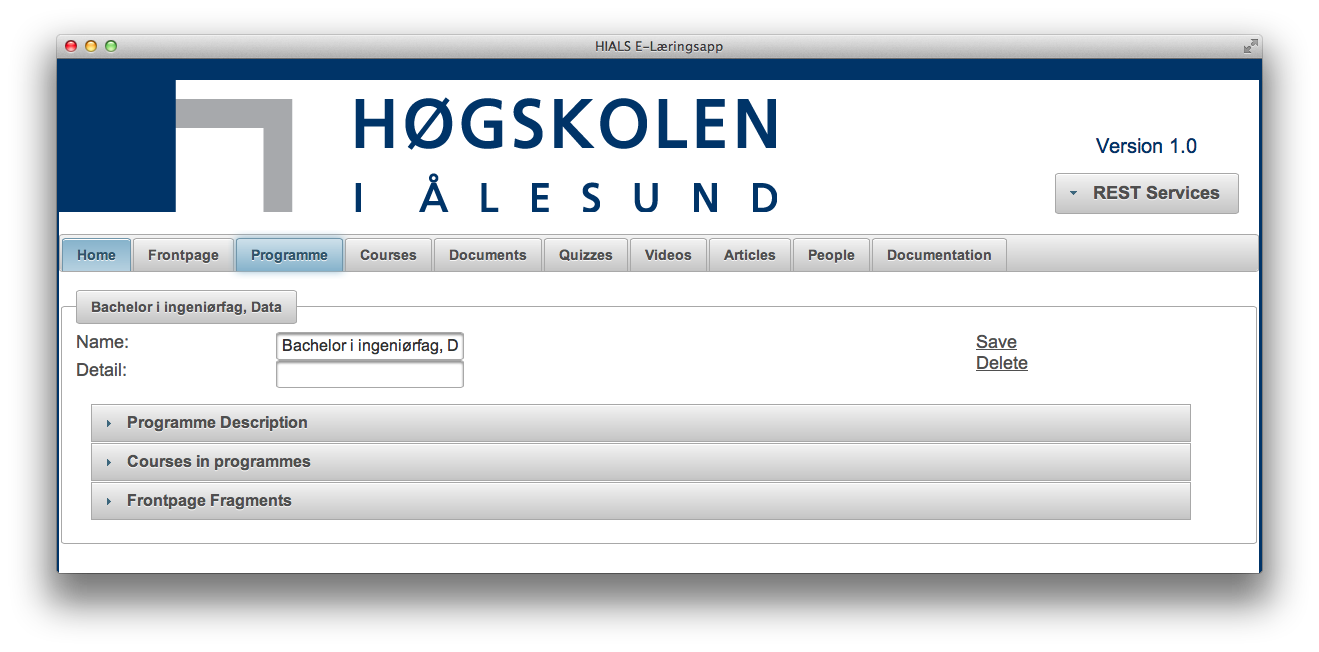
\includegraphics[width=12cm]{webapp_studie.png}
  \caption{Skjermbilde av webapplikasjonen - Studie-redigeringssiden}
\end{figure}

Redigeringssiden for studier. Her kan studiets navn og brødtekst defineres. Resten av siden er delt inn i tre seksjoner

\begin{figure}[H]
  \centering
  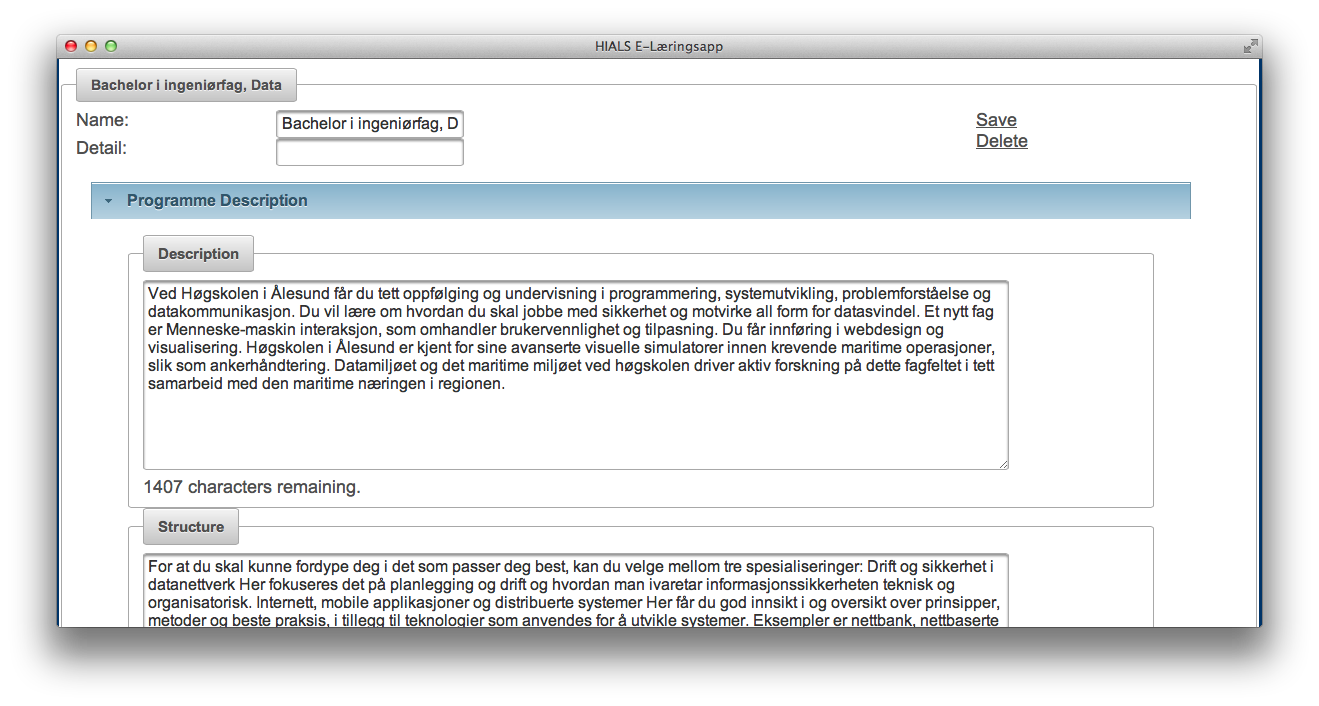
\includegraphics[width=12cm]{webapp_studie2.png}
  \caption{Skjermbilde av webapplikasjonen - Studie-redigeringssiden - Studiebeskrivelse}
\end{figure}

I studie beskrivelsesseksjonen kan mer detaljert tekst om studiet skrives inn.

\begin{figure}[H]
  \centering
  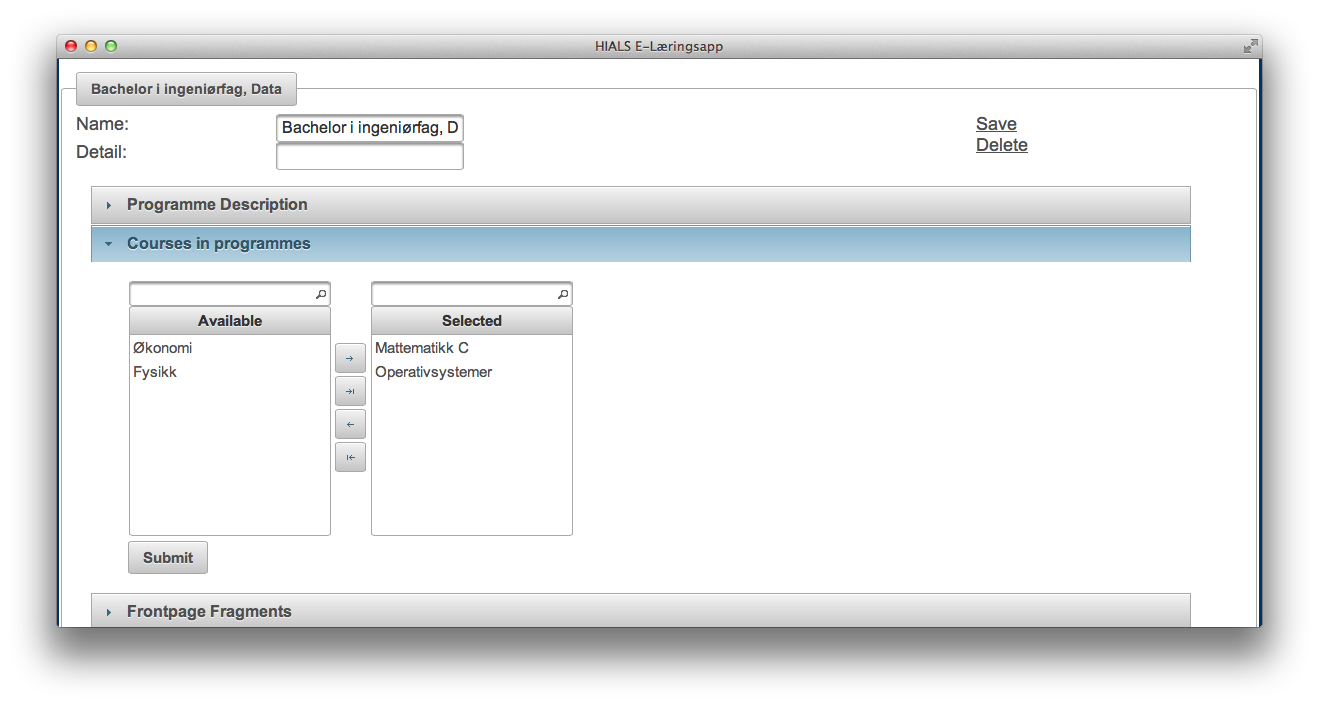
\includegraphics[width=12cm]{webapp_studie3.png}
  \caption{Skjermbilde av webapplikasjonen - Studie-redigeringssiden - Valg av fag}
\end{figure}

Her velger administratoren hvilke fag som er i studiet.

\begin{figure}[H]
  \centering
  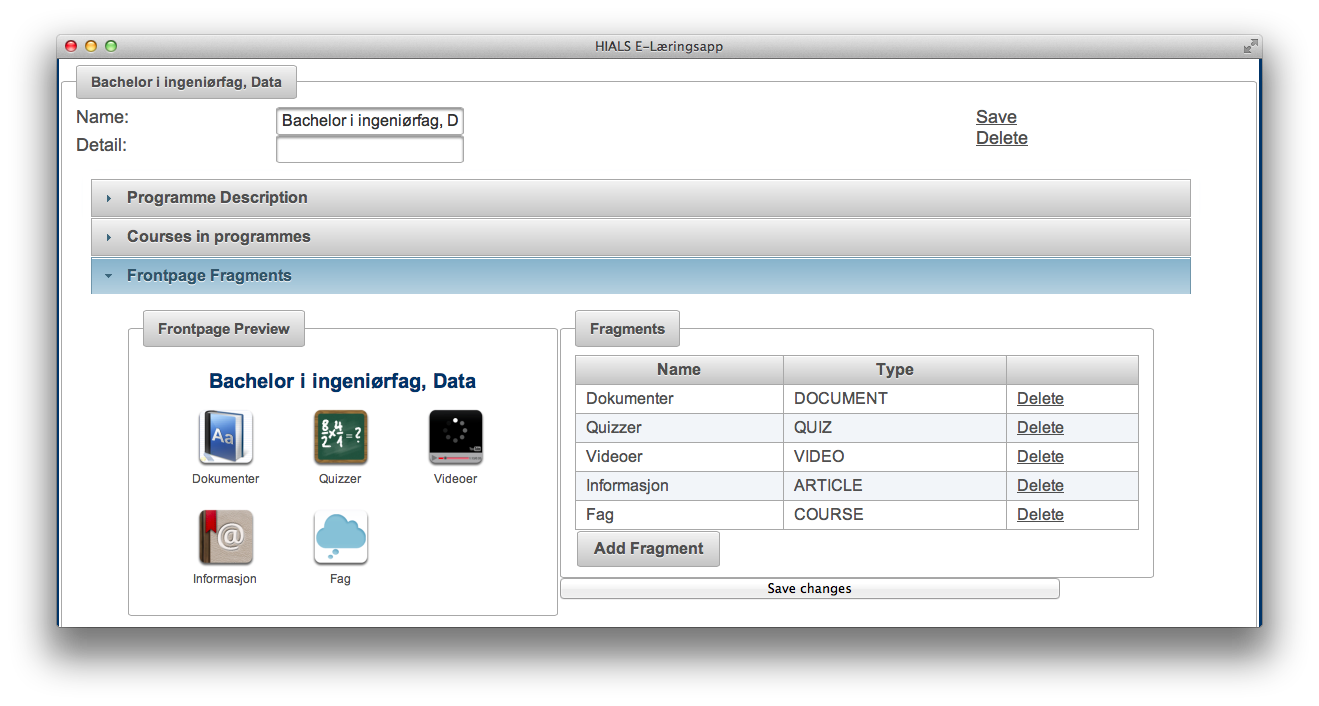
\includegraphics[width=12cm]{webapp_studie4.png}
  \caption{Skjermbilde av webapplikasjonen - Studie-redigeringssiden - Fragmenter}
\end{figure}

Her velges fragmentene som skal visest for det valgte studiet i mobilapplikasjonen.

\subsubsection{Fag}

\begin{figure}[H]
  \centering
  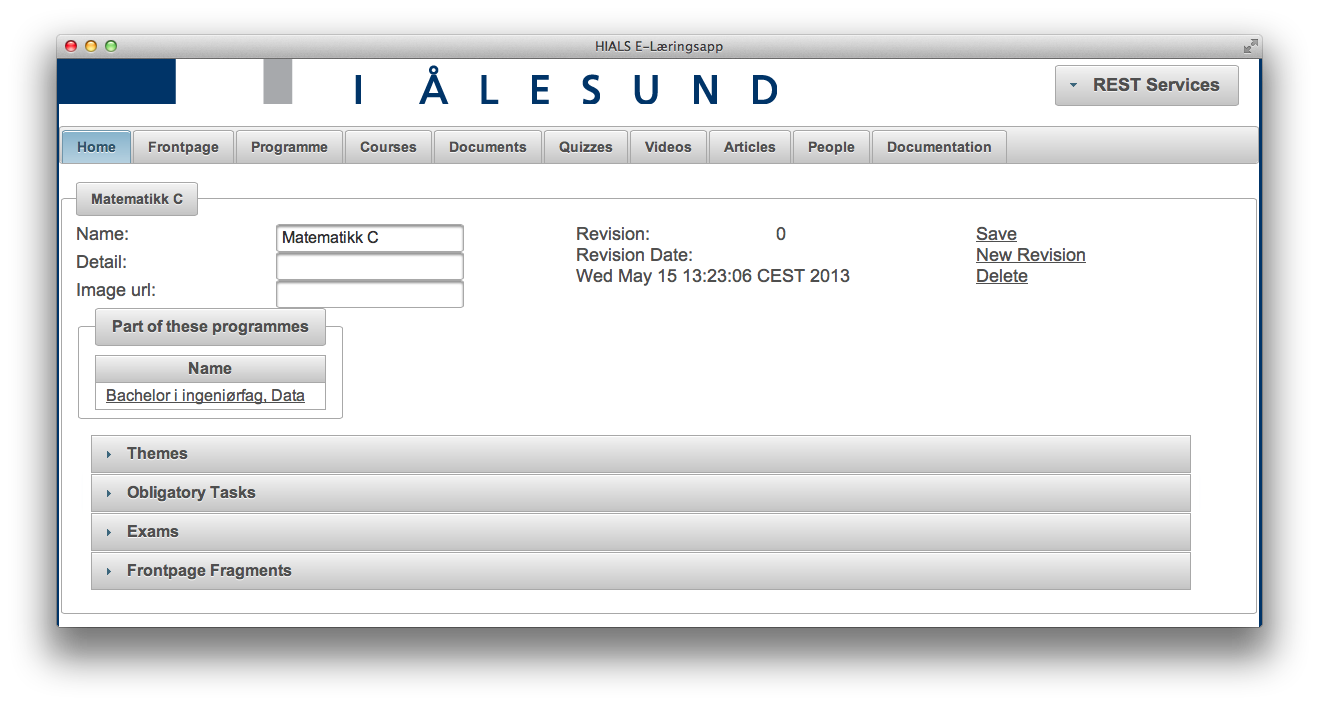
\includegraphics[width=12cm]{webapp_fag.png}
  \caption{Skjermbilde av webapplikasjonen - Fag-redigeringssiden}
\end{figure}

Redigeringssiden for fag. Her defineres fagets navn, brødtekst og bilde. Her visest også hvilke studier faget tilhører. Resten av siden er delt inn i underkategorier der fagets tema og oppgaver, obligatoriske innleveringer, eksamener og hvilke fragmenter som skal vises på mobilapplikasjonen defineres.

\subsubsection{Dokumenter}
Som i de andre fanene vises først alle dokumentene i systemet i en liste.

\begin{figure}[H]
  \centering
  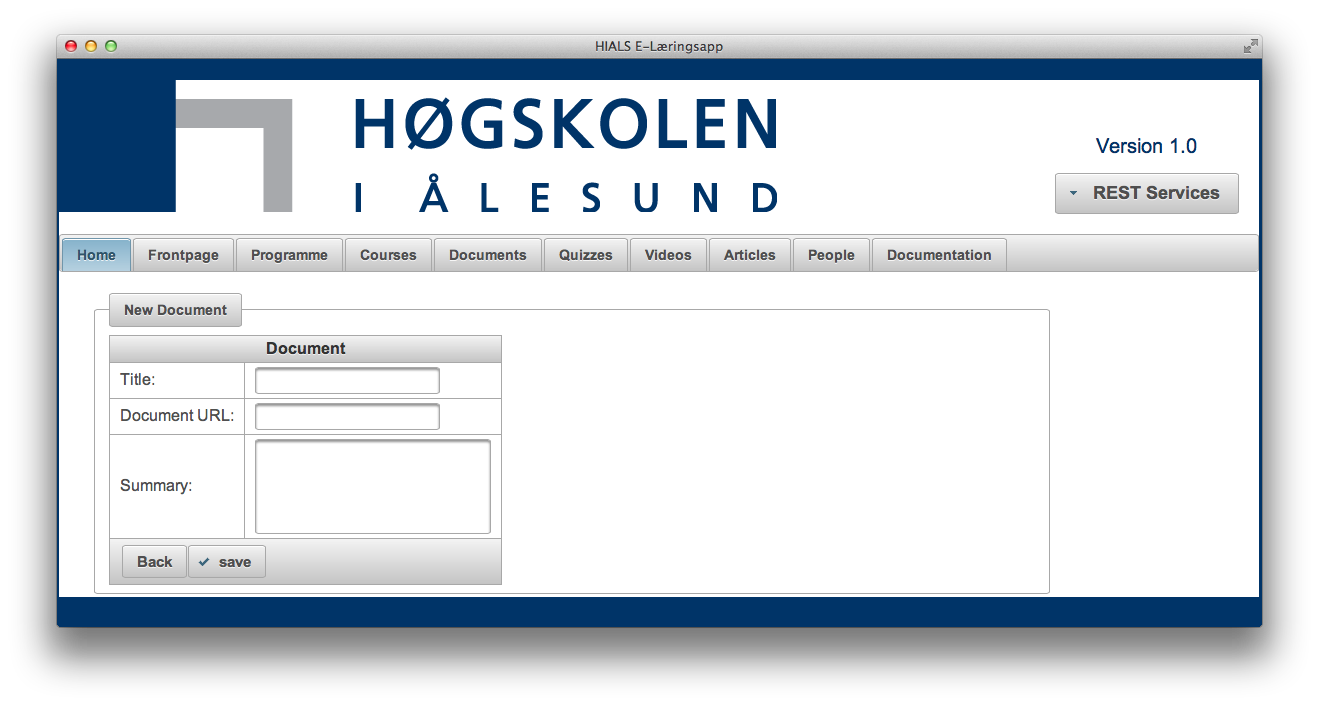
\includegraphics[width=12cm]{webapp_dokument.png}
  \caption{Skjermbilde av webapplikasjonen - Dokument-redigeringssiden}
\end{figure}

Redigeringssiden for dokumenter. Her legges inn navnet til dokumentet, URL eller lenke til dokumentet (i denne versjonen av systemet er ikke filopplasting / lagring støttet, derfor må filene lastes opp til en annen server/tjeneste og linkes til) og en liten tekstbeskrivelse av dokumentet.

\subsubsection{Quizzer}

Som vanlig vises først en liste over alle quizzen i systemet.

\begin{figure}[H]
  \centering
  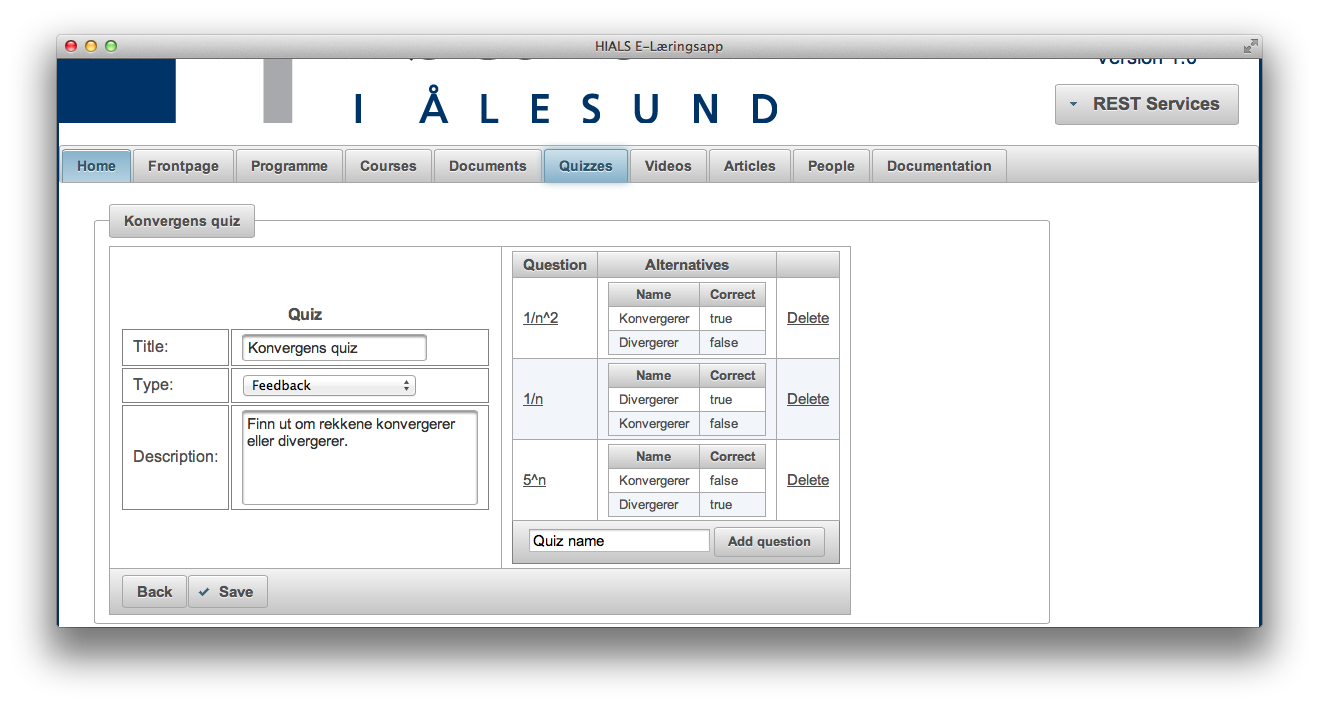
\includegraphics[width=12cm]{webapp_quiz.png}
  \caption{Skjermbilde av webapplikasjonen - Quiz-redigeringssiden}
\end{figure}

Redigeringssiden til en quiz. Her defineres quizzens tittel, type, en kort beskrivelse og spørsmålene med alternativer. Typene quiz er feedback, remote, remote med feedback og guide. Meningen med disse forskjellig typene er som følge

\begin{table}[H]
\begin{center}
\caption{Viser de forskjellige quiz typene}
  \begin{tabular}{ | p{5cm} | p{8cm} |}
    \hline
    Quiztype & Mening \\ \hline
    Feedback & Brukeren får vite resultatet på quizzen \\ \hline
    Remote & Brukeren får ikke vite resultatet på quizzen, men det blir sendt til læreren/forelesere \\ \hline
    Remote med feedback & Brukeren får vite resultatet på quizzen, og resultatet blir sendt til læreren/forelesere \\ \hline
    Guide & Her avhenger hvert spørsmål av det forrige. På denne måten kan man dirigere brukeren mot for eksempel riktig studieretning etc \\
    \hline
  \end{tabular}
\end{center}
\end{table}

Av disse typene er det kun feedback som er ferdig implementert grunnet tidshensyn. De andre typene ligger der da de er delvis implementert og kan gjøres ferdig i fremtide

\begin{figure}[H]
  \centering
  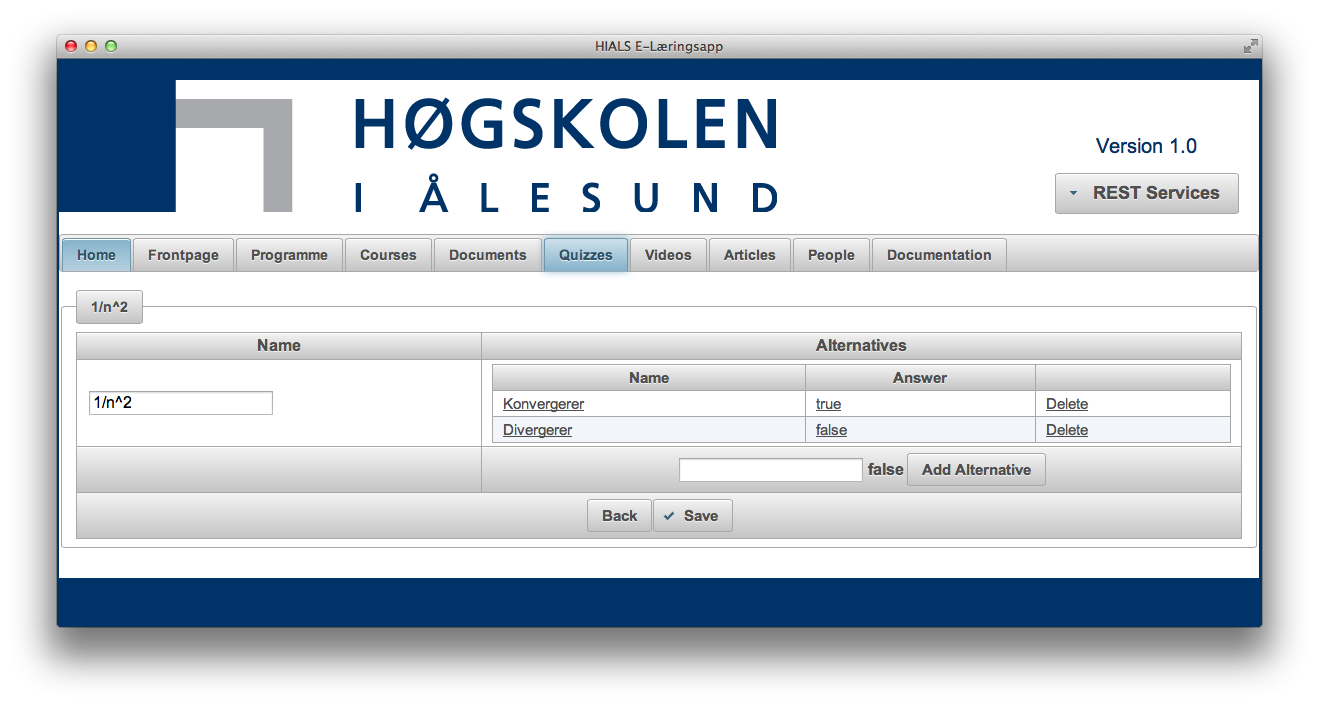
\includegraphics[width=12cm]{webapp_quiz2.png}
  \caption{Skjermbilde av webapplikasjonen - Quiz-redigeringssiden - Spørsmål}
\end{figure}

Redigeringssiden til et valgt spørsmål. Her kan administratoren legge til alternativer og velge hvilke som er riktig svar.


\subsubsection{Videoer}
Først vises en liste over alle videoene i systemet.

\begin{figure}[H]
  \centering
  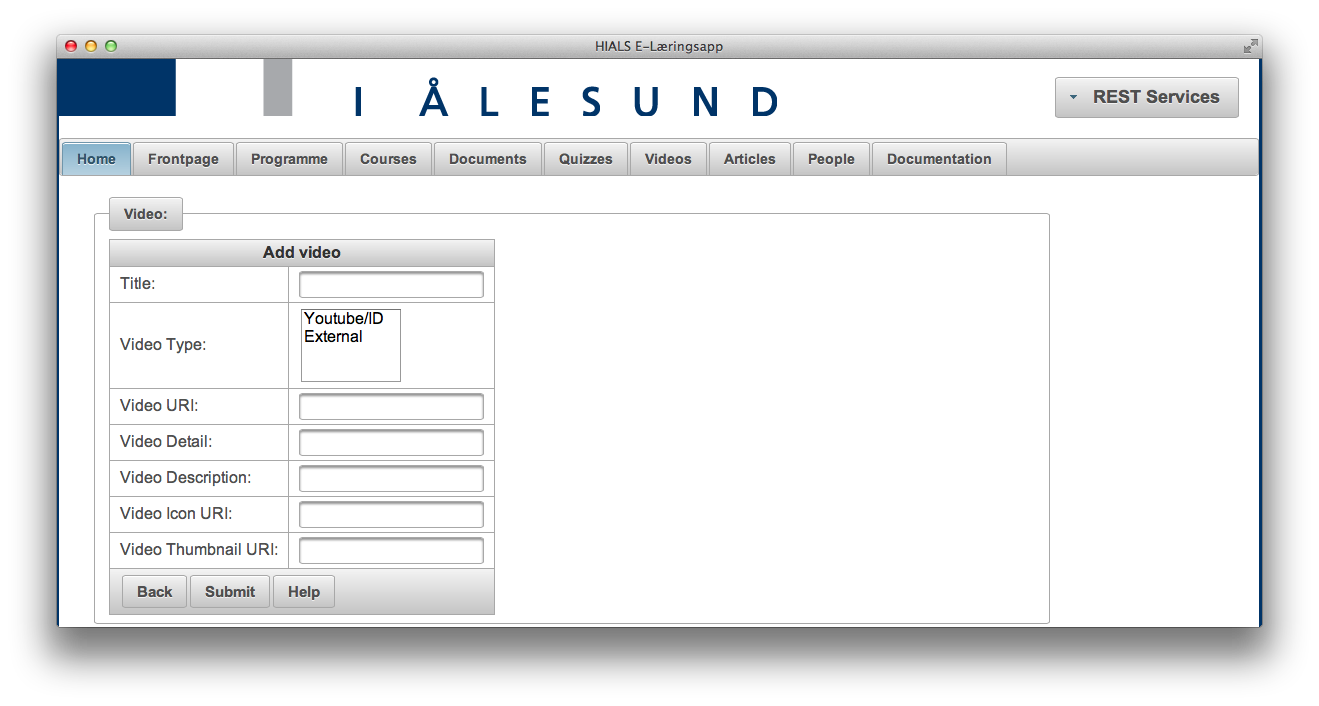
\includegraphics[width=12cm]{webapp_video.png}
  \caption{Skjermbilde av webapplikasjonen - Video-redigeringssiden}
\end{figure}

Redigeringssiden for videoer. Her legges inn / redigeres navnet til videoen, typen (youtube eller videofil), URL / link til videoen, brødtekst, beskrivelse, URL til bildefil for videoens ikon i mobilapplikasjonens listevisning og et thumbnail bilde


\subsubsection{Artikler}
Som vanlig vises en liste over alle artiklene i systemet.

\begin{figure}[H]
  \centering
  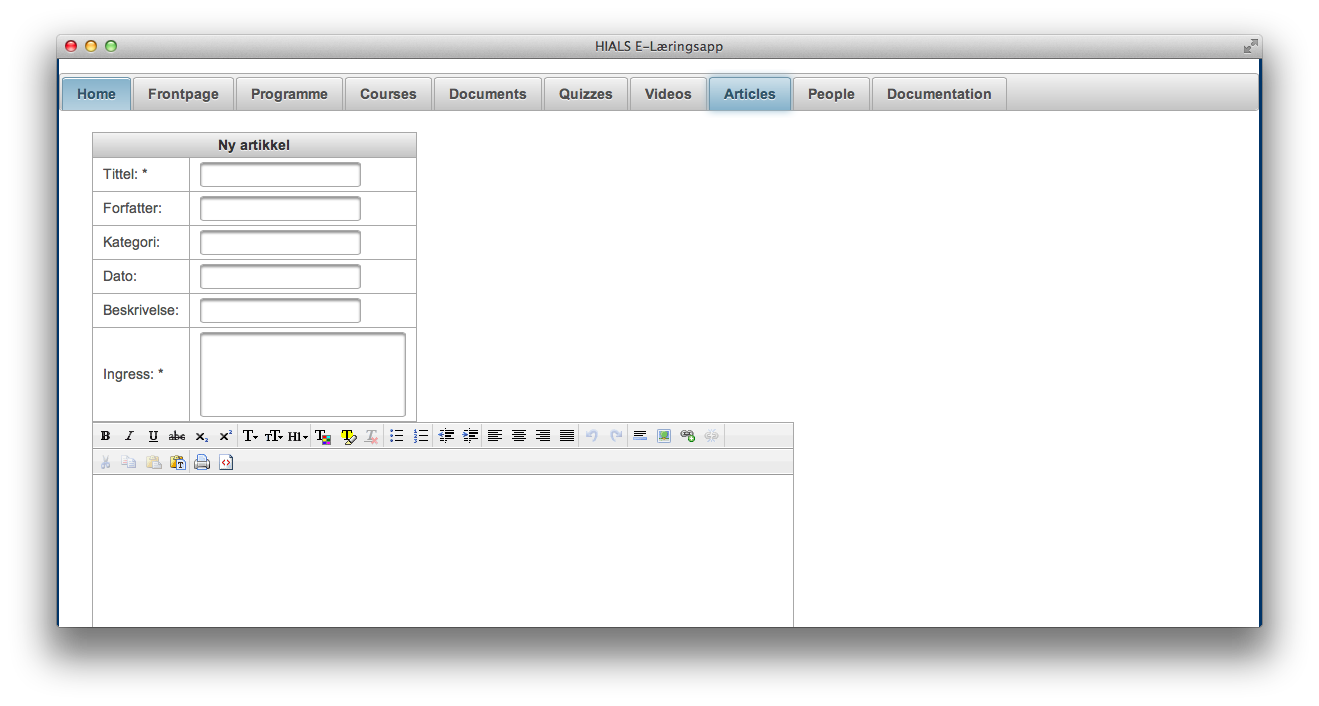
\includegraphics[width=12cm]{webapp_artikkel.png}
  \caption{Skjermbilde av webapplikasjonen - Artikkel-redigeringssiden}
\end{figure}

Redigeringssiden for artikler. Her legges inn / redigeres artikkelens tittel, forfatter, kategori (brukt til å sortere artikler for nyhetsfunksjonen), dato, beskrivelse, ingresstekst og selve artikkelen. Artikkelens tekst bruker en WYSIWYG editor og lagrer artikkelen i HTML format. Administratoren kan også legge inn egendefinerte HTML kode. Stien til artikkel siden er: “server.no/faces/article.xhtml?articleid=<ID>” der <ID> er artikkelens interne I


\subsubsection{Brukere}
Viser en liste over brukerene i systemet.

\begin{figure}[H]
  \centering
  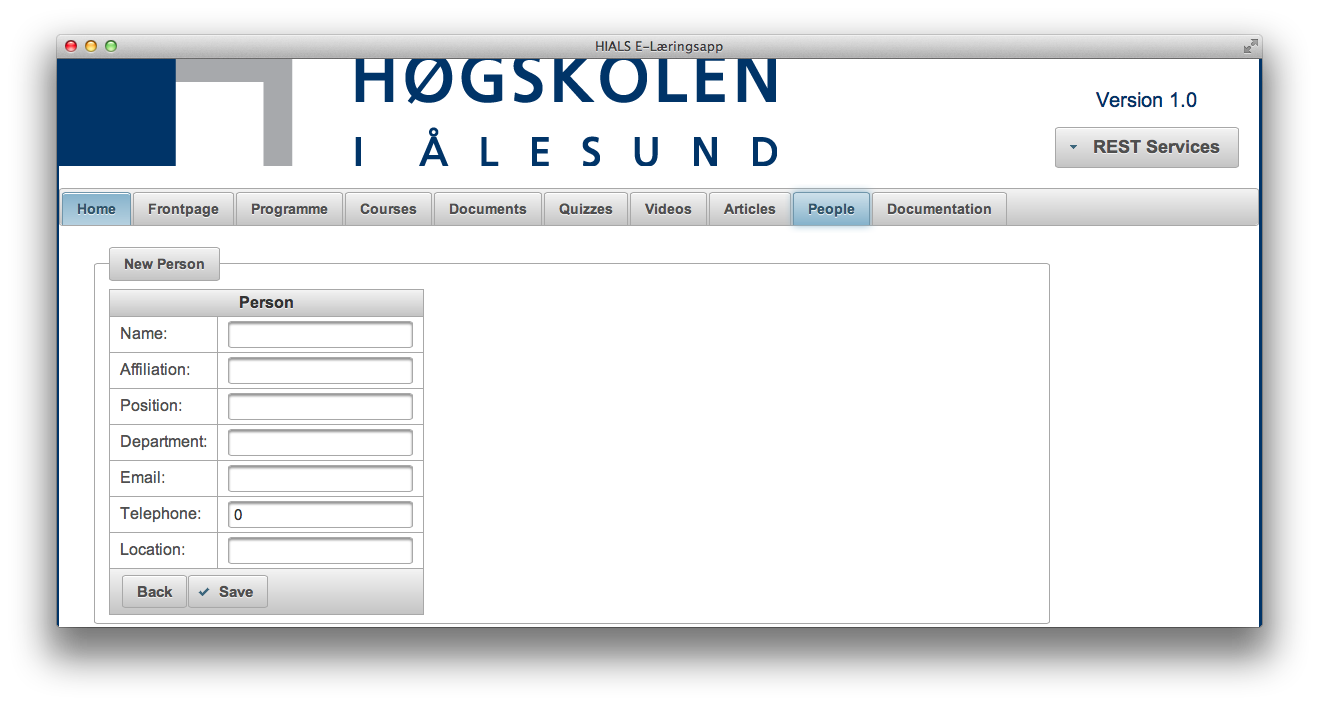
\includegraphics[width=12cm]{webapp_bruker.png}
  \caption{Skjermbilde av webapplikasjonen - Bruker-redigeringssiden}
\end{figure}

Redigeringssiden for brukere. Her fylles inn diverse informasjon om brukeren. I denne versjonen av applikasjonen har brukersystemet ingen funksjon. Brukerfunksjonen var planlagt som både et brukersystem med rettigheter og eierskap av objekter i systemet, og som et oppslagsverk for lærere / ansatte i skolen for skolens eleve

\subsubsection{Dokumentasjon}

\begin{figure}[H]
  \centering
  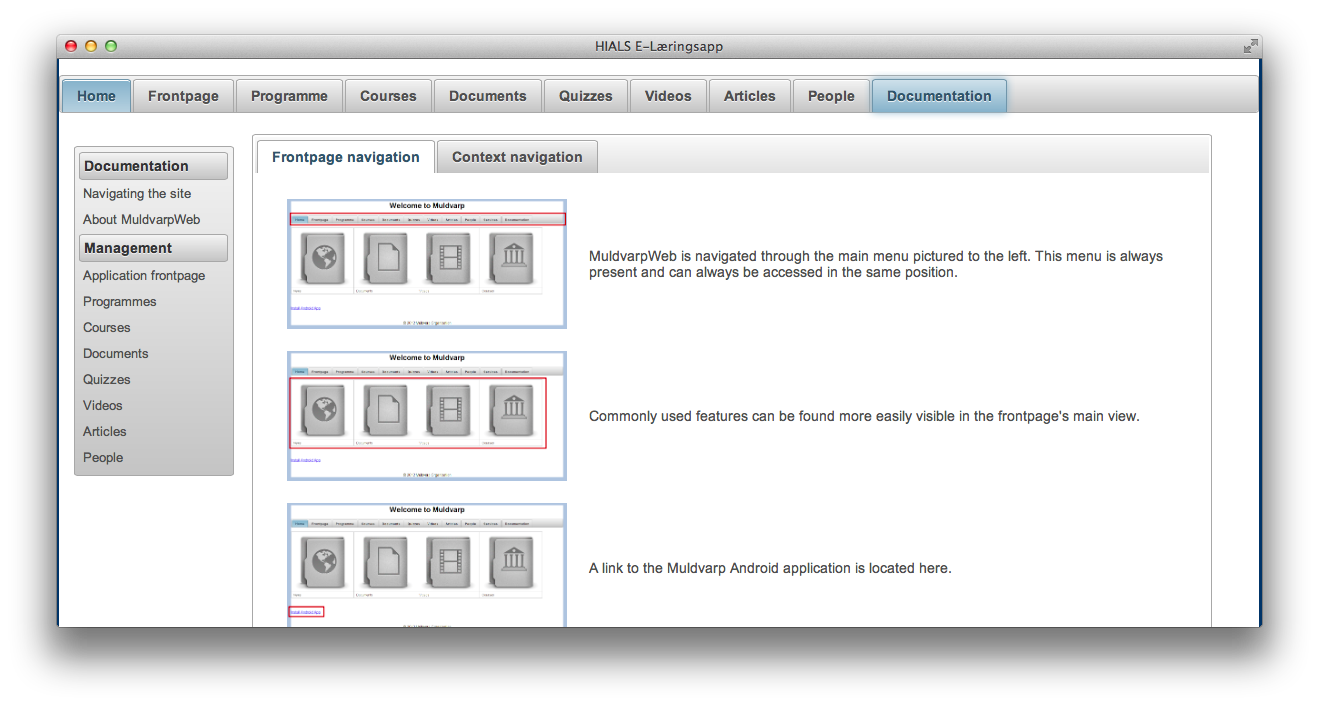
\includegraphics[width=12cm]{webapp_dokumentasjon.png}
  \caption{Skjermbilde av webapplikasjonen - Dokumentasjon}
\end{figure}

Hjelpeside for webapplikasjonen. Her finnes instruksjoner for bruk av de forskjellige delene av administrasjonsgrensesnittet.


\subsection{Modulært fragmentsystem}

I tidligere versjoner av mobilapplikasjonen var fragmentene (se begreper) eller sidene på hvert lag statisk programmert inn i mobilapplikasjonen. I dette systemet hadde alle objektene på et lag (fremside, studieretninger, fag) de samme sidene, en av hvert type fragment. Det var ikke alle tilfellene dette passet med objektets tilgjengelige informasjon, og derfor ble det besluttet at sidene på hvert objekt skulle bli styrt av webapplikasjonen. Med det nye systemet kan administratorene definere nøyaktig hva som skal vises på mobilapplikasjonen. Dette systemet var også laget for å kunne lett utvides med nye moduler. Se kapittelet om mobilapplikasjonen for oversikt over de forskjellige fragmentene

\subsection{ER modell}

\begin{figure}[H]
  \centering
  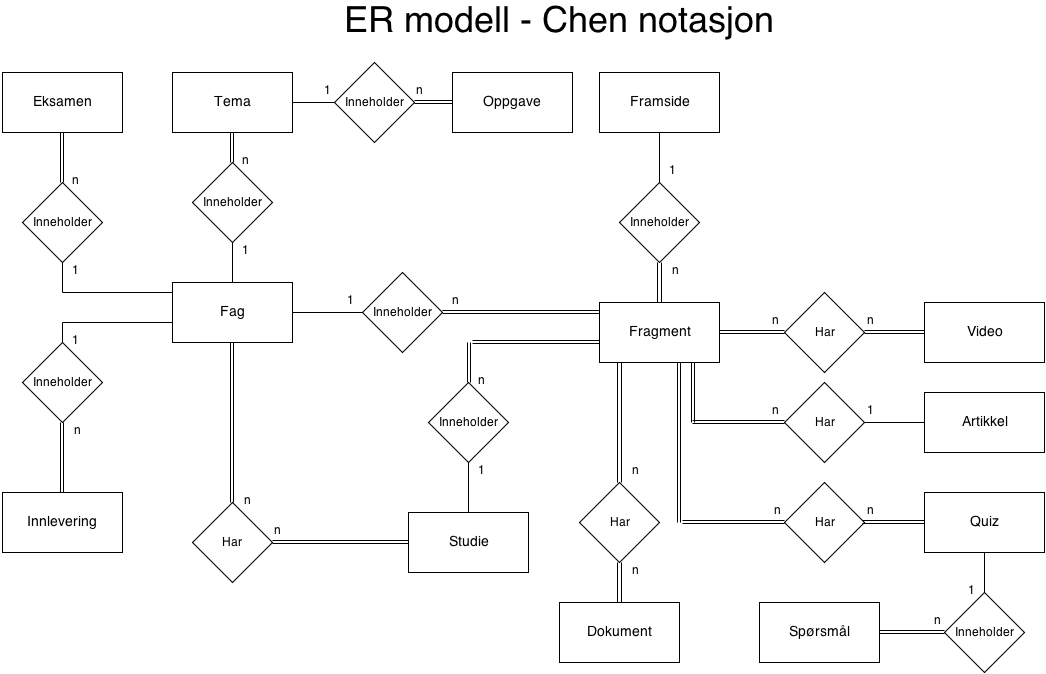
\includegraphics[width=14cm]{ER-modell.png}
  \caption{Entity Relationship diagram}
\end{figure}

ER modellen er bygd opp med det logiske lagene på topp (fremside, studier, fag) der hver av disse inneholder dynamiske fragmenter, som igjen inneholder data objektene (artikler, dokumenter, videoer osv). Topplagene er knyttet til fragmenter via “one to many” relasjon som betyr at for eksempel et studie har flere unike fragmenter. Fragmentene er knyttet til data objektene med “many to many” relasjon. Dette vil si at for eksempel flere fragmenter kan være knyttet til de samme videoene og omvendt.\newline
\newline
I det gamle systemet hadde hvert av lagene (fremside, studie, fag) relasjoner direkte til dataobjektene. Det vil si at hvert lag hadde en instans av hvert fragment. Med det nye fragmentsystemet kan hvert lag ha flere instanser av samme type fragment.

\subsection{REST tjenester}

For at eksterne applikasjoner som mobilapplikasjonen skal kunne bruke dataen i systemet har vi et sett med “RESTful” tjenester. Disse leverer begrenset informasjon basert på hva klientapplikasjonen spør om. Her er en oversikt over hvilke tjenester som er i bruk av denne versjonen av applikasjonen.

\begin{table}[H]
\begin{center}
\caption{Viser de tilgjengelige REST tjenestene}
  \begin{tabular}{ | p{5cm} | p{8cm} |}
    \hline
    URL/Forespørsel (domene.no/services/ + & Data / respons \\ \hline
    frontpage & Henter fremsiden \\ \hline
    programme & Henter alle studier \\ \hline
    programme/<ID> & Henter studiet med valgt ID \\ \hline
    articles/news & Henter artikler med kategori “news” \\ \hline
    course/<ID> & Henter kurset med valgt ID \\ \hline
    article/<ID> & Henter artikkel med valgt ID \\ \hline
    timeedit/coursecode/<kode> & Henter timeplanen for valgt fagkode (eks ID102012) \\ \hline
    timeedit/classcode/<kode> & Henter timeplanen til valgte klasse (eks DA1) \\ \hline
    bibsys/<Søkeord> & Finner alle bøker som matcher søkeordet \\ \hline
    fronter/room/<ID> & Hente data fra fronter rom med ID (siden fronter implementasjonen ikke ble fullført returnerer dette bare dummy data) \\
    \hline
  \end{tabular}
\end{center}
\end{table}





\section{Systemintegrasjon}

\subsection{TimeEdit}

Den første oppgaven ved integreringen av TimeEdit var å bestemme hvilke av tjenestene som TimeEdit tilbyr var nyttig for applikasjonen’s bruksområde. TimeEdit som implementert av HIALS tilbyr bla. 

\begin{itemize}
\item Booking av rom. \endnote{\url{https://timeedit.hials.no/WebReservations/WebObjects/}} \newline
Krever HIALS brukernavn/passord
\item Timeplan over planlagte forelesninger \endnote{\url{http://timeedit.hials.no/4DACTION/WebShowSearch/1/1-0?}} \newline
 ….basert på :
\begin{itemize}
\item Studieløp
\item Enkeltfag
\item Forelesere
\item Rom
\end{itemize}
\end{itemize}

Hovedfokuset i applikasjonen er sentrert rundt studier og enkelt-fag, og dermed er den mest relevante tjenesten oppslag på nettopp dette. TimeEdit kan supplere den eksisterende funksjonaliteten i mobil-applikasjonen ved å tilby dypere innsikt i og bredere oversikt over studier og enkeltfag. Mer konkret skal en bruker av mobil-applikasjonen være i stand til å slå opp et fag eller studie, og så ha muligheten til å få servert en ferdig formatert og relatert time-plan.
Det å kunne enkelt reservere rom fra applikasjonen er forsåvidt også noe som har klar nytteverdi, men er ikke like godt knyttet opp mot applikasjonen’s hovedfokus. Dermed ble booking av rom ikke tatt med i funksjonsimplementeringen.

\subsubsection{Utvikling}

Når hvilke tjenester fra TimeEdit som skulle implementeres i applikasjonen ble fastslått, gjensto det å bestemme metoden for å oppnå integreringen. Denne delen beskriver hvilke valg-alternativ vi kom fram til at vi hadde, sammenligning og den endelige vurderingen.\newline
\newline
TimeEdit er som tidligere beskrevet en tjeneste utviklet av selskapet Evolvera som tilbys brukeren gjennom en nettleser. Basert på kun denne kunnskapen kunne vi ramse opp tre metoder for å implementere skolens timeplanløsning i applikasjonen. Disse tre (med begrunnelse) er:
\begin{enumerate}
\item Bruk av eksisterende API tilknyttet TimeEdit\newline
For en slik data-sentrert tjeneste er det sannsynlig at en API-løsning er utviklet, da dette er vanlig for moderne geskjefter. \endnote{Matthew A.Russel,  O’Reilly Media, Inc, 2011, Mining the Social Web}
\item Web-scraping av HIALS TimeEdit’s nettside\newline
Som beskrevet i delen om Web-Scraping under Teoretisk Grunnlag, er det mulig å parse en nettside for relevant data og rekonstruere den i et mer anvendbart format.
\item Vise TimeEdit’s nettside direkte gjennom Android’s eksisterende funksjoner\newline
Dette er et klart valg-alternativ som er gjennomførbart.
\end{enumerate}

En oppsummeringsliste med ulemper/fordeler ved disse valgmulighetene er tilgjengelig lengre nede i denne seksjonen, i tillegg til hvilken som ble valgt. \newline
\newline
Av disse tre alternativene er direktevisning av TimeEdit’s nettside enklest å implementere, da dette kun innebærer å lage en container i applikasjonen(ved bruk av Android WebView) som peker til siden. Ulempen med denne metoden er at nettsiden til TimeEdit ikke er designet for visning på små skjermer. Dette innebærer at det må mye navigering (zooming, scrolling, leting) til for å komme fram til riktig data, noe som er lite ønskelig fra et brukerperspektiv.\newline
Gruppen benyttet Galaxy Nexus-enhetene til å besøke og navigere HIALS TimeEdit’s nettside, med dårlig brukeropplevelse som forventet. Dataene var presentert uoversiktlig og de små skjermene gjorde det vanskelig å utbedre dette. Dermed ble det tidlig klart at å vise TimeEdit’s nettside direkte var langt i fra et ønskelig alternativ, selv om tilnærmings-metoder som det å bruke en WebView til å ha en egen-definert CSS-fil for å endre layout ble inkludert i vurderingen. \newline
Trolig kunne vi ha fått til bedre visning på små skjermer, men dataene ville likevel vært utilgjengelig for oss dersom vi ikke benyttet oss av web-scraping-teknikker for å strukturerere de.\newline
\newline
Den foretrukne metoden er å bruke TimeEdit’s eget API. Ved bruk av et API vil applikasjonen være tildels beskyttet mot små forandringer i koden til TimeEdit, og dataene ville kunne bli presentert i applikasjonen med det samme gjennomgående utseende/temaet som de andre funksjonene. Ulempene med denne metoden i forhold til å bare vise nettsiden til TimeEdit er at det er noe mer arbeid å grafisk presentere dataene i applikasjonen.\newline
Web-scraping er det mest tidkrevende av de tre alternativene fordi det legger til ekstra steg med arbeid for å få hentet ut dataene. I tillegg til å hente og presentere dataene, er det nødvendig å utvikle en metode for å filtrere ut kun riktig data fra TimeEdit’s nettsider. En annen ulempe er at løsningen er sårbar for forandringer på TimeEdit sine nettsider.
Basert på det ovennevnte kan vi hevde følgende fordeler og ulemper:

\begin{enumerate}
\item Bruk av eksisterende API tilknyttet TimeEdit\newline
+ Sikker\newline
+ Allerede utviklet og ummiddelbart anvendbar\newline
-  Avhengig av en tredjepart\newline
\item Web-scraping av HIALS TimeEdit’s nettside\newline
+ Mer frihet til å definere løsning\newline
-  Usikker\newline
-  Tidkrevende da ekstra arbeid er nødvendig\newline
\item Vise TimeEdit’s nettside direkte\newline
+ Enklest å implementere\newline
-  Kanskje vanskeligst å implementere godt\newline
-  Lite presenterbar på mobile applikasjoner\newline
-  Ingen kontroll eller strukturering av relevante dataene\newline
\end{enumerate}

Etter å ha vurdert disse tre metodene ble gruppen enige om å bruke TimeEdit’s API. Grunnlaget for dette er at det fremsto som det alternativet som ville enklest gi oss et strukturert datasett å jobbe med, da både alternativ 2 og 3 krever web-scraping for å ekstrahere nyttig data. Hvis dataene var allerede tilgjengelig i et API kunne mye arbeid unngås. Enkeltheten ved å vise TimeEdit’s nettside direkte så ikke ut til å være verdt presentasjonsproblemene som ville forekomme. Dermed følger prioriteringen for ønsket metode samme nummerering som listen i figuren.

For å gå frem med denne løsningen tok vi kontakt med Geir Halsvik, som er leder for IT seksjonen ved Høgskolen i Ålesund. Av han fikk vi vite at ansvarlig for TimeEdit ved høyskolen er Nils Roald, og at systemet driftes av Kenneth Opedal. Vi ble også informert om at skolen er i gang med å implementere en stor oppdatering av TimeEdit systemet. Den nye versjonen av TimeEdit(versjon 3.x) vil bli betydelig forskjellig fra dagens utgave, både på frontend og backend.\newline
\newline
Dette gjør at vi møter en ny problemstilling - skal applikasjonen lages for dagens system, og bli avleggs om noen måneder, eller skal vi prøve å få tak i tilgang til den nye versjonen? Gruppen ble enige om å kontakte Evolvera(de som utvikler systemet) ångående API for den nye versjonen. Etter første runde med undersøkelser fikk vi vite at det er nødvendig med en sertifisering for å få tilgang til systemet. Etter dette bestemte gruppen seg for å ta kontakt med Evolvera direkte, da et slikt kurs ville måtte ta sted i Sverige, og gruppen har hverken tid eller ressurser til et slikt kurs. I mellomtiden skulle gruppen utforske web-scraping som et alternativ i tilfelle det ikke var mulig å få API tilgang uten kurs. Som en siste utvei kan problemet løses ved å presentere TimeEdit sin nettside i applikasjonen. Dette har fordelen med at man kan bare forandre ressurslinken når det nye systemet kommer i drift. Ulempen med dette er at nettsidene ikke er tilpasset liten skjerm som diskutert tidligere.\newline
Forsøk på aksessere TimeEdit’s API uavhengig av noe kurs for sertifisering med prøving-og-feiling i nettleseren lyktes heller ikke.\newline
\newline
Løsningen som ble valgt var å implementere en web-scraping-mekanisme på serversiden av applikasjonen som tilbød strukturert data gjennom et egetutviklet API (web service). Mobil-applikasjonen er i stand hente de dataene den trenger fra web-applikasjonen ved behov. Dette løser også problemstillingen med at HIALS skulle implementere en ny versjon av TimeEdit, da det ikke blir nødvendig å oppdatere samtlige mobile enheter for å kompensere for endringen. For brukerne vil ikke opplevelsen bli noe forskjellig med den gamle TimeEdit løsningen og den nye TimeEdit løsningen.

\subsection{Lovlige hensyn}

Med den løsningen som ble valgt var det viktig å vite at innhentingen av dataene ikke bryter med noen lover om opphavsrett, da spesifikt åndsverksloven \endnote{\url{http://www.lovdata.no/all/tl-19610512-002-001.html\#1}}.
Etter å ha undersøkt dette, hovedsakelig ved bruk av internett kom vi frem til konklusjonen at innhentingen av data ikke bryter med lover eller retningslinjer for opphav av data. Dette er basert på de to følgende argumentene;

\begin{itemize}
\item Dataene er produsert og administrert av skolen, og er derfor skolens eiendom. Evolvera(selskapet som leverer og eier TimeEdit), leverer kun løsningen som presenterer dataene.
\item Robots.txt filen som ligger ved timeplanen tilsier at automatiske tjenester kan innhente data fra alle kataloger for domenet timeedit.hials.no\endnote{\url{http://timeedit.hials.no/robots.txt}}. Dette er en vedlagt fil/protokoll som viser hva automatiske tjenester har tilgang til.
\end{itemize}



\subsection{Utvikling av løsning}

Da det var bestemt at vi skulle benytte oss av web-scraping for å søke etter og hente ut behandlingsklar informasjon, begynte vi med analyse av TimeEdit-tjenesten som tilbudt sluttbrukeren via nettsiden \endnote{\url{http://timeedit.hials.no/4DACTION/WebShowSearch/1/1-0?wv\_type=5\&wv\_search=\&wv\_startWeek=1301\&wv\_stopWeek=1318\&wv\_first=0}}.

\begin{figure}[H]
  \centering
  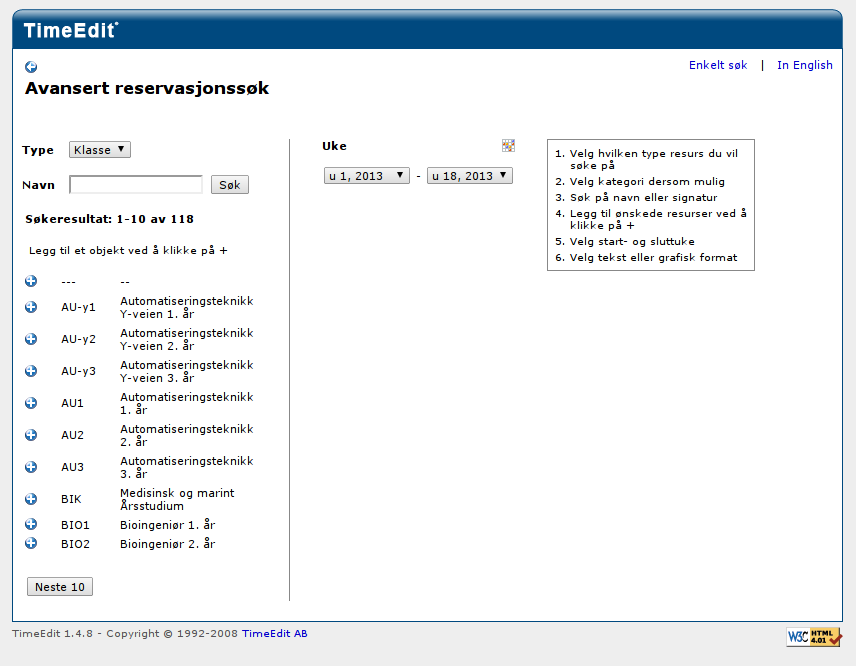
\includegraphics[width=14cm]{timeedit1.png}
\caption{Ovenfor  er et skjermbilde av TimeEdtit’s nettside for søk på klasser}
\label{fig:TimeEditMain}
\end{figure}
Nettsiden i Figur 1.31 er grensesnittet til tjenesten som vi skal integrere. Den er aksesserbar fra hvilkensomhelst nettleser via HIAL's hjemmeside \endnote{\url{http://www.hials.no}} og inneholder de funksjonene fra TimeEdit som vi ønsker å integrere i e-læringsapplikasjonen. Selve dataene vi ønsker befinner seg i tekstformat i en eller annen del av kildekoden. Kildekoden kan granskes enkelt ved hjelp av en nettleser eller ved å laste ned siden og åpne den med et tekstredigeringsprogram. Vi benyttet oss av nettleseren for å granske kildekoden. Kildekoden består av svært mye tekst, og det vil ikke legges ved denne rapporten, men kan undersøkes ved å laste ned nettsiden selv. Der det er nødvendig vil vi vise utdrag.\newline
\newline
Ved å se nærmere på kildekoden finner man at nettsiden består av standard HTML, og benytter seg av Javascript for å endre side-innhold via å manipulere og sende input-parametere via HTML-forms. 

\begin{lstlisting}[language=HTML, frame=single, caption={Utdraget av HTML kildekoden til TimeEdit ovenfor viser en JavaScript-funksjon og en input-tag.}]
function addObject(id) {
var reloadingdiv = document.getElementById('reloading');
reloadingdiv.style.display = '';
document.form.wv_addObj.value = id;
document.form.submit();

.......

<INPUT type='hidden' name='wv_addObj' value=
\end{lstlisting}

Dette foregår ved at brukeren interagerer med elementer i nettsiden (knapper, søkefelt (input forms) o.l) som er bundet tl JavaScript funksjoner. På denne måten kan nettleseren tolke brukeren's ønsker, og TimeEdit vil svare med mer HTML og JavaScript som inneholder en timeplan. Bruker-input lagres som parametere i HTML input-forms som tolkes som parametere ved sending. Disse parameterene sendes med HTTP GET, og dette betyr at bruker-inntastet data er synlig i URL'en. Det er da enkelt å hente ut ønsket innhold uten å måtte benytte seg av Javascript eller å hente innhold mer enn en gang. Ønskede parametre kan settes som strenger i etter den eksisterende URLen, og ønsket innhold kan hentes direkte dersom man har kjennskap til strukturen. På denne måten unngår vi bruk av TimeEdit's nettside helt. \newline
Neste steg er derfor å skaffe seg kjennskap til og forståelse av strukturen i TimeEdit's nettleser-baserte tjeneste. Selve dataene som TimeEdit leverer og dets struktur (timeplan) må forstås, i tillegg til strukturen i det underliggende systemet og hvordan URL'en kan manipuleres for å levere resultatet som inneholder dataene vi trenger.

\begin{figure}[H]
  \centering
  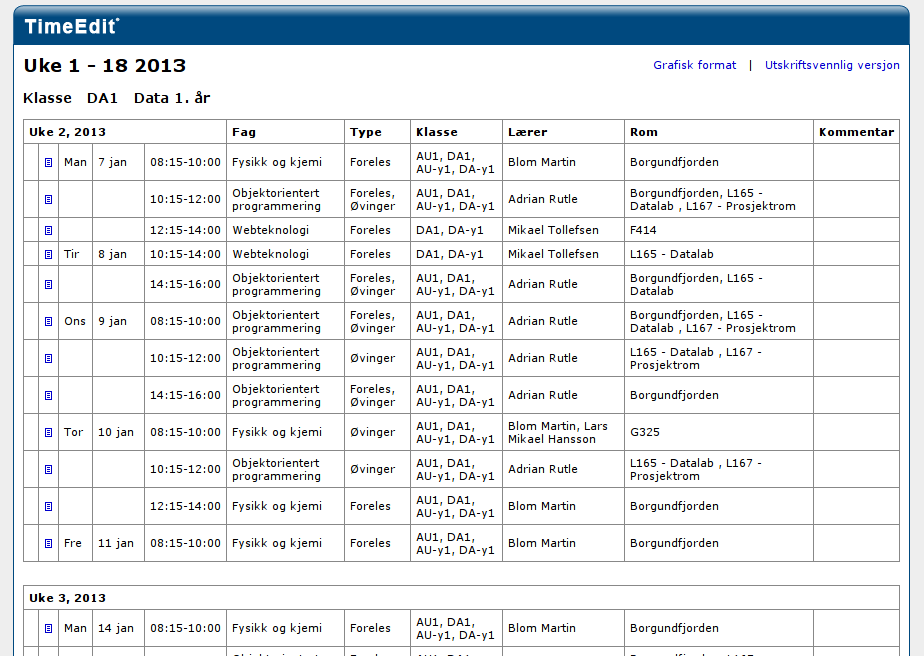
\includegraphics[width=14cm]{timeedit2.png}
  \caption{En vanlig timeplan}
\end{figure}

I selve timeplanen som presentert av TimeEdit, kan oversikts-perspektivet brytes ned i følgende tidsgrupperinger:

\begin{enumerate}
\item År (semestertimeplan)
\item Uker
\item Dager
\item Forelesninger (Tidsramme definert av klokkeslett)
\end{enumerate}

Forelesningene er det meste relevante for visining i E-lærings-applikasjonen og inneholder også det meste av informasjonen som knyttes opp til applikasjonen’s innhold. (Fag, Studieløp etc)
Dette utgjør måldataene som vi må produsere en metode for å pålitelig kunne hente ut.\newline
\newline
Neste steg var å finne ut hvordan TimeEdit’s programstruktur gjør seg synlig via nettsiden, og hvordan dette kunne benyttes.

\begin{figure}[H]
  \centering
  
\includegraphics[width=5cm]{timeedit3.png}
\caption{Treff-element som vises etter søk i TimeEdit som presentert i en nettleser.}
\end{figure}

\begin{lstlisting}[language=HTML, frame=single, caption={Utdrag av kildekoden til TimeEdit's nettside som vist i figur 1.32}]
<a href='javascript:addObject(175000)'><img src='/img/plus.gif' ...>
\end{lstlisting}

Av kildekoden til TimeEdit og det assosierte elementet i nettleseren ovenfor, kan vi resonnere oss fram til at enheter i systemet som fag, lærere eller klasser er i systemet representert som objekt med tilhørende datafelt. Felles for alle objektene er en ID bestående utelukkende av tall på fem eller seks siffer som benyttes for å kunne gjøre oppslag i systemet. Dette ser vi fra JavaScript funksjonen i figur 1.33. Disse informasjonsobjektene representerer f.eks fag, klasser eller rom, og danner grunnlaget for hvordan timeplanen skal formateres. Vi kan videre resonnere oss fram til at TimeEdit har dermed et eget system for håndtering og kontroll av informasjonsobjekter. Dette systemet ser ikke ut til å være direkte kompatibelt med systemet i E-lærings websiden eller Høyskolens andre systemer. Dette var forventet av gruppen, men presenterer også ett problem som må under utviklingen løses for at systemene skulle kobles sammen sømløst. Problemet er at vi ikke kan gjøre oppslag eller søk i TimeEdit's system med unike data-felt i vårt eller Høyskolen's system. \newline
Det neste steget går ut på å analysere URLen som brukes for å hente svar fra HIALS TimeEdit's server. URL'en påvirker direkte svar-resultatet og kan i seg selv definere hva som skal hentes uten noe behov for å sende med ett objekt eller lignende. Nedenfor er en slik URL:

\begin{lstlisting}[language=HTML, frame=single, caption={En URL generert når man søker etter en timeplan for ett spesifikt fag}]
http://timeedit.hials.no/4DACTION/WebShowSearch/1/1-0?wv_type=5&wv_ts=20130511T191704X3729&wv_search=&wv_startWeek=1301&wv_stopWeek=1318&wv_first=0&wv_addObj=&wv_delObj=&wv_obj1=174000&wv_text=Tekstformat
\end{lstlisting}

Man kan lese av URL’en og analysere de forskjellige parameterene. Parameterene er forøvrig alt som befinner seg etter spørsmålstegnet i URL'en, og består av nøkkel-verdi par bundet sammen med likhetstegn. En parameter er separert fra en annen med tegnet ampersand. Selve parameterene med tilhørende verdier er skrevet på engelsk eller norsk, og disse ordene er forkortelser eller sammensetninger som også forteller om parameterens bruksområde.  I tillegg matcher parameternavnene funksjonsnavnene i Javascript, som også gir videre grunnlag for å bestemme hva de gjør. Med enkel deduksjon og noe prøving og feiling, finner man fram hvilke parametre som gjør hva, hvilken rekkefølge de må stå i, og hvilke som er nyttige for E-lærings-applikasjonens bruk.

\begin{table}[H]
\begin{center}
\caption{Tabell over parametere i URLen separert som navn og verdi med tilhørende funksjon}
  \begin{tabular}{ | p{3cm} | p{6cm} | p{6cm} |}
    \hline
    Navn & Verdi & Funksjon \\ \hline
    wv\_type & Tall & Bestemmer hvilket type objekt som skal søkes etter. \newline Fag/Kurs = 3 \newline Klasse/Program = 5 \newline Foreleser = 6 \newline Rom = 7 \\ \hline
    wv\_ts & Dato + Streng & Sesjon \\ \hline
    vw\_search & Streng & Søk på navn tilhørende objekt \\ \hline
    vw\_startWeek & Streng bestående av 4 tall, siste to siffer fra år og ukenummer. & Bestemmer når timeplanen skal starte. \\ \hline
    vw\_stopWeek & Streng bestående av 4 tall, siste to siffer fra år og ukenummer. & Bestemmer når timeplanen skal stoppe. \\ \hline
    vw\_obj1 \newline (inkluderer wb\_obj2, \newline wb\_obj3 etc) & Tall-streng bestående av fem eller seks siffer. & Setter hvilke objekt i TimeEdit systemet som skal inkluderes i timeplanen. \\ \hline
    vw\_text & Spesifikk tekst-streng: \newline tekstformat \newline grafisk \newline tekst & Bestemmer hvordan timeplanen skal representeres. \\ \hline
    vw\_addObj & Tall-streng bestående av fem eller seks siffer. & Legger til ett objekt til listen. \\ \hline
    vw\_delObj & Tall-streng bestående av fem eller seks siffer. & Fjerner ett objekt fra listen. \\
    \hline
  \end{tabular}
\end{center}
\end{table}

Tabellen ovenfor ble utarbeidet ved å bruke TimeEdit's nettside i en nettleser, gjøre endringer og observere hva som blir endret, fjernet eller lagt tili URLen. Av parameterene ovenfor er har kun ett fåtall noen nytteverdi for vår bruk, noe som er svært heldig da det vil gjøre jobben med å implementere en løsning mindre komplisert. Vi vil med første øyekast kun ha bruk for parameterene som velger objekt for visning i TimeEdit-systemet, og parameterne som velger tidsrammen for timeplanen. Videre testing viser at de nødvendige parameterene vi må benytte må stå i følgende rekkefølge:

\begin{enumerate}
\item wv\_obj1
Objektkoder går først, så mange som nødvendig (obj1, obj2 etc...).
\item startWeek, stopWeek
Disse er valgfrie, men bør defineres for enkelhets skyld.
\item vw\_text
\end{enumerate}

Med denne kunnskapen er det mulig å konstruere en URL som returnerer en ønsket timeplan gitt at man kan objektkoden tilhørende faget eller studieløpet i TimeEdit-systemet. 

\subsubsection{Valg av teknologi/støttebibliotek}

Følgende den initielle analysen av TimeEdit’s presentasjonslag, gjenstår implementasjon av web-scraping løsning i server-delen av web-applikasjonen.  Løsningen må benytte Java, være i stand til å hente ut og analysere web-sider samt være godt nok dokumentert til å kunne enkelt endres ved behov. Kravet for å enkelt kunne endres var nødvendig for å kunne svare på eventuelle endringer i Time-Edit systemet.
I tillegg til en selv-utviklet løsning som benytter Java's HTTPClient pakke, eksisterer følgende løsninger utviklet av tredjeparter myntet på nettopp web-scraping:

\begin{itemize}
\item Jsoup \endnote{\url{http://jsoup.org}}
\item TagSoup \endnote{\url{http://home.ccil.org/~cowan/XML/tagsoup/}}
\item HTMLUnit \endnote{\url{http://htmlunit.sourceforge.net/}}
\item Web Harvest \endnote{\url{http://web-harvest.sourceforge.net/}}
\item jArvest \endnote{\url{http://sing.ei.uvigo.es/jarvest/examples.html}}
\end{itemize}

Tanken på utvikle en egen løsning via Java’s eget HTTPClient bibliotek falt bort da det er mye enklere og tidsbesparende å benytte en eksisterende løsning som allerede er godt dokumentert. Noe testing med en egen løsning ble utført, men det skapte en større kodebase å vedlikeholde, noe som ikke var ønskelig og heller ikke nødvendig i dette tilfellet. Ved å lære og bruke en av de ovennevnte støttebibliotekene kunne gruppen dermed fokusere på den viktigste delen av løsningen - selve uthentingen og bearbeidingen av informasjonen.\newline
\newline
Gruppen som helhet analyserte de forskjellige alternativene som nevnt i listen ovenfor ved å gå gjennom dokumentasjon og presentasjon av funksjonalitet som bibliotekene hadde. Disse er alle nettbaserte.
Gruppen konkluderte med at Jsoup var det enklest benyttbare alternativet. En av de viktigste grunnene til at gruppen kom til denne beslutningen var at Jsoup viste seg å være best dokumentert, fra både offisielt hold og tredjeparts bruk av Jsoup. 
En annen og minst like viktig grunn, var hvordan gruppen oppfattet enkelheten i syntaksen. For eksempel HTMLUnit imiterer en klient, og krever gjerne dypere kjennskap til kildekoden som skal analyseres, og har litt mer komplisert og noe for ordrik syntaks. For å f.eks hente ut en spesifikk tag i et HTML-dokument krevde HTMLUnit for mye.
Jsoup og TagSoup imiterer HTML-hierarkiet på en logisk måde i kode-syntaksen, noe som gjorde det mer attraktivt en andre alternativer (Objektstrukturen i biblioteket hadde et hierarki som etterlignet HTML-hierarki-systemet).Dette ville gjøre koden mer lesbar, vedlikeholdbar og ikke minst skrivbar for gruppemedlemmene. 

\subsubsection{TimeEdit og E-læringsapplikasjonen, to forskjellige systemer}

En metode for å kunne sette likhetstegn mellom to objekter i to forskjellige systemer, f.eks et fag som representert av E-lærings websiden og et fag som representert av TimeEdit var som tidligere nevnt nødvendig.\newline
\newline
TimeEdit støtter også søk med fritekst, og søk med fagkode eller klassekode gir som regel ett resultat som vist i bildet nedenfor - dette kan vi utnytte til å hente ut TimeEdit-objektkodene vi trenger.

\begin{figure}[H]
  \centering
  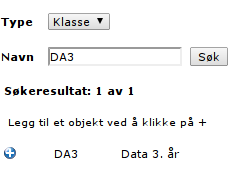
\includegraphics[width=5cm]{timeedit4.png}
  \caption{TimeEdits fritekstsøk for fag og klasse}
\end{figure}

Som vist i figur (vis til tidligere kodesnipp her) inneholder treff-elementet objektkoden, og herfra er det kun et spørsmål om hvordan man skal legge til dette søkesteget i løsningen.

\subsubsection{Utvikling av løsning i Java med Jsoup og JAX-RS}

Basert på analysen av TimeEdit og ved valg av støttebibliotek gjensto det kun å utvikle løsningen konkret. 

\subsubsection{Generering av URL}

Basert på det som kom fram av analysen av TimeEdit tidligere, opprettet vi funksjoner som genererte en korrekt formatert URL basert på relevante input-parametere.

\subsubsection{Parsing i Jsoup}
Med Jsoup som støttebibliotek kan henting, parsing og REST-funksjonalitet skrives inn i en og samme klasse, en EJB om nødvendig. Jsoup er kompakt, funksjonsrikt og lettbrukt nok til at dette er mulig uten å gjøre koden uleselig. For å beholde modulariteten i systemet, utviklet vi TimeEdit-løsningen som en enkelt støttet REST root resource klasse, som beskrevet i seksjonen Teoretisk Grunnlag - REST tjenester. Et utdrag fra denne klassen er vist nedenfor:

\begin{lstlisting}[language=Java, frame=single, caption={Kodesnipp fra klassen TimeEditService, som er grovt kortet ned.}]
......
import javax.ejb.Stateless;
import javax.ws.rs.GET;
import javax.ws.rs.Path;
import javax.ws.rs.PathParam;
......
@Stateless
@Path("timeedit")
public class TimeEditService {
    //Maximum number of object requests that will be parsed by getURL()
    private static int MAX_OBJECT_REQUESTS = 10;
.......
}
\end{lstlisting}

I første omgang var det viktigst å få gjort en tilkobling via HTTP til TimeEdit for å få hentet ut et HTML-dokument og skape en logisk struktur av de nødvendige dataene som kunne behandles programmatisk. For å få til en slik struktur, ble en del indre klasser opprettet for representere forskjellige objekter som speilet TimeEdit’s innordning av objekter og tidsrammer. Disse klassene er kun nyttig i sammenheng med midlertidig organisering av data, og har ikke nytte utenfor klasse-skopet.

TimeEditSchedule \newline Representerer ett år med semesterplaner.
\begin{itemize}
\item ScheduleWeek \newline Klasse som representerer ett sett med dager.
\begin{itemize}
\item ScheduleDay \newline Klasse som representerer en dag i timeplanen med forelesninger.
\begin{itemize}
\item ScheduleLecture \newline Klasse som representerer en forelesning for ett gitt kurs.
\begin{itemize}
\item ScheduleCourse \newline Klasse som representerer en forelesning for ett gitt kurs.
\end{itemize}
\end{itemize}
\end{itemize}
\end{itemize}

En forbindelse mellom vår EJB og TimeEdit er enkelt opprettet som illustrert av kode-utraget nedenfor:

\begin{lstlisting}[language=Java, frame=single, caption={Et utdrag av en metode i TimeEditService som viser hvordan Jsoup benyttes for å hente ut ett enkelt dokument}]
public TimeEditSchedule getTimeEditSchedule(String siteURL){      
        TimeEditSchedule timeEditSchedule = new TimeEditSchedule();
        Document doc = null;
        ......
        try {
            doc = Jsoup.connect(siteURL).get();
        } catch (IOException ex) {
            Logger.getLogger(TimeEditService.class.getName()).log(Level.SEVERE, null, ex);
        }      
\end{lstlisting}

Document-objektet doc kan så enkelt gjennomgås ved hjelp av løkker og if-setninger som utnytter vår kjennskap til kildekoden til HTML-dokumentet som returneres av TimeEdit. Eksempelet nedenfor viser hvordan man kan gå gjennom HTML via Jsoup og hente ut data:

\begin{lstlisting}[language=Java, frame=single, caption={asdasdsadasdasdasdsadsadasdasdsadsa}]
if(!tableColumns.get(i).getElementsByTag("font").isEmpty()){
                  stringData = tableColumns.get(i).getElementsByTag("font").first().text();
                  if(stringData.contains("Uke")){
                              //create new week and break loop if the first element contains Uke
//                            System.out.println("NEW WEEK: " + stringData);
.....
}
\end{lstlisting}

HTML-dokumentet som returnert av TimeEdit sorterer informasjonen vi trenger ved hjelp av standard tabeller med rader og kolonner. Framgangsmetoden vi benyttet for å hente ut dataene gikk dermed ut på å gå gjennom hver rad og hente ut tekstdataene i hver kolonne. Som demonstrert i figur (vis til tidligere figur her) er informasjonen av lik type i alle samsvarende kolonner - dvs at i envher rad vil f.eks kolonne nummer 5 alltid vil inneholde samme type data.
Hovedtabellen er merket med en class-tag (“booking”), og med Jsoup hentes tabellen enkelt ut og man kan iterere over innholdet og ekstrahere data med en switchcase nummerert etter hver kolonne. Noe forkortet illustrasjon fra funksjonen getTimeEditSchedule nedenfor:

\begin{lstlisting}[language=Java, frame=single, caption={asdasdsadasdasdasdsadsadasdasdsadsa}]
.....
 Element content = doc.getElementsByClass("booking").first();
            Elements rows = content.getElementsByTag("tr");
            for(Element row : rows) {
                Elements tableColumns = row.getElementsByTag("td");
                for(int i = 0; i < tableColumns.size(); i++) {
.....
switch(i){
                                case 2: //Dag (Man, Tir, Ons etc)
                                    day = new ScheduleDay(stringData);
                                    break;
.....
}
\end{lstlisting}

\begin{lstlisting}[language=HTML, frame=single, caption={asdasdsadasdasdasdsadsadasdasdsadsa}]
<TABLE class='booking' border='0' cellpadding='5' cellspacing='0'>
\end{lstlisting}

Med dette fikk vi organisert hele timeplanen inn i en struktur som vi senere kunne behandle programmatisk.  

\subsubsection{Spørring på fagkode og klassekode}

Som tidligere nevnt var det også nødvendig å kunne hente ut en timeplan basert på fagkode eller klassekode. Dette løste vi ved å bruke to HTTP-spørringer, ett for å finne riktig TimeEdit objektkode basert på TimeEdit’s fritekstsøk, og ett siste for å hente ut den faktiske timeplanen som benyttet metoden vi har utviklet tidligere.

\begin{lstlisting}[language=Java, frame=single, caption={asdasdsadasdasdasdsadsadasdasdsadsa}]
@GET    @Path("coursecode/{coursecode}{startweek:(/startweek/[^/]+?)?}{stopweek:(/stopweek/[^/]+?)?}{date:(/date/[^/]+?)?}")
    @Produces({MediaType.APPLICATION_JSON})
    public Response getScheduleByCourseCode(@PathParam("coursecode") String courseCode,
            @PathParam("startweek") String startweek,
            @PathParam("stopweek") String stopweek,
            @PathParam("date") String date) {
        
        System.out.println("course code: " + courseCode);
        String[] objectCodes = getObjectCodeFromCourseCode(courseCode).split("/");
        System.out.println("objectCode[0]: " + objectCodes[0]);
        return getResponse(objectCodes, date, startweek, stopweek, true);
    }
\end{lstlisting}

\begin{lstlisting}[language=Java, frame=single, caption={asdasdsadasdasdasdsadsadasdasdsadsa}]
public String getObjectCodeFromQuery(String query, int type){
        String searchURL = TIMEEDIT_HIALS_URL + TIMEDIT_PARAM_SEARCH_TYPE + "=" + type + "&" + TIMEDIT_PARAM_SEARCH + "=" + query;        Document doc = null;
        try {
            doc = Jsoup.connect(searchURL).get();
        } catch (IOException ex) {
            Logger.getLogger(TimeEditService.class.getName()).log(Level.SEVERE, null, ex);
        }
        Elements elements = doc.select("a");
        System.out.println("Elements size: " + elements.size());
        Pattern pattern = Pattern.compile("javascript:addObject\\((\\d{6}|\\d{7})\\)");
        Matcher matcher;
        for(Element e : elements){
            String currentString = e.attr("href");            if(currentString != null && !currentString.isEmpty()){
                matcher = pattern.matcher(currentString);
                if(matcher.find()){                    String retVal = matcher.group().replace("javascript:addObject(", "");
                    retVal = retVal.replace(")", "");
                    return retVal;
                }
            }
        }
        return "";
    }
\end{lstlisting}

Ovenfor er en funksjon fra TimeEditService som utfører en HTTP-forbindelse via Jsoup til TimeEdit, og bruker Java’s regex-bibliotek til å finne å identifisere søketreffene som inneholder riktig TimeEdit-kode. Som vist i kapittelet om analyse av TimeEdit, befinner TimeEdit-koden seg som variabel inne i et kall til en javascript-funksjon. Da vi har navnet til denne funksjonen, “addObject()”, trenger vi regex til å matche denne funksjonen. Dette ble fullført med regex-strengen under:

\begin{lstlisting}[language=HTML, frame=single, caption={asdasdsadasdasdasdsadsadasdasdsadsa}]
javascript:addObject\\((\\d{6}|\\d{7})\\)
\end{lstlisting}

Som vil matche all tekst som inneholder denne javascript-funksjonen, og som et ekstra lag med sikkerhet kun variabler som har en lengde på seks eller sju siffer. I java regex noterer “\\d” et tall, hvorav etterfølgende krøllparanteser ({}) med som inneslutter et tall noterer lengde. I sammenheng med symbolet “|” som betyr “OR”, velger vi da å matche innhold med enten seks eller sju siffer.
Etter dette kan man enkelt skrelle vekk teksten i javascript-funksjonen og hente ut selve tallet (TimeEdit objektkode) med Java’s String replace-funksjon.
Deretter kan man benytte den samme metoden vi utviklet for å hente ut timeplaner basert på objektkoder. Videre skulle det også å ha vært mulig å lagre klasse-kode og TimeEdit objektkodene, slik at det kun ville ha vært nødvendig å gjøre to HTTP-spørringer en gang for hver kode, eller muligens kjøre gjennom alle fagkodene for å hente ut TimeEdit objektkodene. Dette kunne oppnås ved å legge til ett felt i Course og Programme JPA-klassene som representerer en TimeEdit kode. 

\subsubsection{Design av API}
Denne delen omhandler hvilke grunnlag vi la til rette for å utvikle vår API for TimeEdit samt hvilke resultater vi endte opp med.

\subsubsection{API}
API’et er utviklet kun med tanke for bruk av e-læringsapplikasjonen for mobile plattformer. Med dette blir dokumentasjon og svar-type mindre viktig og arbeidet kan fokuseres på å kunne produsere riktige og konsistente resultater. Det blir heller ikke nødvendig å produsere svar i mer enn en type dataformat, og gruppen ble enige om å bruke JSON siden det fremstår som mer lettlest og ikke unødvendig ordrikt. Dette betyr midlertidig ikke at flere dataformat kan tilbys om nødvendig i framtiden.

\subsubsection{API-URI}

URI-en til TimeEdit API-et som tilbudt av E-lærings-nettstedet ble utviklet med overflatisk simplisitet og lesbarhet som mål. Dette betyr at man skulle kunne tolke og forstå hva som ønskes søkt av en spørring mot API’et kun ved å lese URI’en uten nødvendigvis å ha dyp kjennskap til API’et. Formålet med dette er å gjøre API’et lett å jobbe opp i mot, og å redusere tiden brukere av API’et benytter for å skaffe innsikt i systemet samt for å redusere tiden brukt til feilsøking da feil vil forhåpentligvis forekomme sjeldnere.\newline
I tillegg skulle eventuelle feiltastinger eller annet feilbruk av API-et ikke taksere det underliggende systemet ved å gjøre unødvendig arbeid med spørringer som ikke vil gi noe nyttig resultat. Klart feilformaterte spørringer burde dermed forkastes, og bruker opplyses om dette.\newline
\newline
For å oppnå disse målsetningene benytter vi oss av Java’s API for REST webservices, JAX-RS. Dette medfølger Java EE, og det er da kun et spørsmål om å gjøre bruk av API’et.
Som tidligere nevnt hadde vi opprettet en REST root resource service klasse (TimeEditService), hvor vi har annotert klassen med @Path og variabel “timeedit”, som gjør den gjeldende ressurs-stien til følgende:

\begin{lstlisting}[language=HTML, frame=single, caption={asdasdsadasdasdasdsadsadasdasdsadsa}]
{server}/services/timeedit/
\end{lstlisting}

Deretter vil enhver funksjon med @Path annotasjon innenfor klasse-skopet benytte ressurs-stien ovenfor, i tillegg til sin egen-definerte variabel.
Basert på behovet som definert tidligere kom vi fram til at API’et måtte tilby minst følgende tjenester:

\begin{itemize}
\item
\begin{itemize}
\item timeedit objekt-koder
\item fagkode
\item klassekode
\end{itemize}
\end{itemize}

I tillegg skulle det være mulig å definere en start-uke og stopp-uke eller dato i timeplanen for å avgrense svar-innholdet.\newline
For å tilfredsstille behovet ovenfor (og evt. ekstra behov), opprettet vi følgende endepunkter for webservices:

\begin{table}[H]
\begin{center}
\caption{DASDSADSADASDASDASDASDASDADASD}
  \begin{tabular}{ | p{4cm} | p{6cm} | p{6cm} |}
    \hline
    Service URI & Funksjonsnavn & Beskrivelse \\ \hline
    /timeedit/ & getScheduleByMultipleObjectID\newline getParams & Aksepterer TimeEdit objektkoder og svarer med fullt formatert timeplan \\ \hline
    /timeedit/simple/ & getSimpleScheduleByMultipleObjectID & Aksepterer TimeEdit objektkoder og svarer med enkelt formatert timeplan \\ \hline
    /timeedit/coursecode/ & getScheduleByCourseCode & Aksepterer kurskoder og svarer med enkelt formatert timeplan \\ \hline
    /timeedit/classcode/ & getScheduleByClassCode & Aksepterer fagkoder og svarer med enkelt formatert timeplan \\ \hline
    /timeedit/params/ & getScheduleByMirrorParameters & Speiler TimeEdit sitt parameter-system, aksepterer også fulle URLer \\ \hline
    /timeedit/query/ & getScheduleByQuery & Ikke implementert \\
    \hline
  \end{tabular}
\end{center}
\end{table}

\begin{figure}[H]
  \centering
  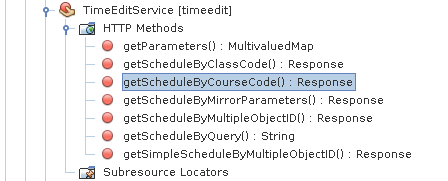
\includegraphics[width=5cm]{timeedit5.png}
  \caption{Demonstrerer Web-servicene som registrert}
\end{figure}

Disse endepunktene vil ikke dekke hele TimeEdit’s funksjonsbredde, men er mer en tilstrekkelig for vår bruk. 

\begin{lstlisting}[language=Java, frame=single, caption={asdasdsadasdasdasdsadsadasdasdsadsa}]
  /**
     *
     * @param id The ID of the Object from which the schedule is to be
     * retrieved. The Object ID can represent a Course (Fag), a
     * Programme(Klasse), or a combination.
     * @param objectString
     * @param startweek
     * @param stopweek
     * @param date
     * @return Response
     */
@GET    @Path("{objectstring:|((\\d{6}|\\d{7})/?)+}{startweek:(/startweek/[^/]+?)?}{stopweek:(/stopweek/[^/]+?)?}{date:(/date/[^/]+?)?}")
    @Produces({MediaType.APPLICATION_JSON})
    public Response getScheduleByMultipleObjectID(@PathParam("objectstring") String objectString,
            @PathParam("startweek") String startweek,
            @PathParam("stopweek") String stopweek,
            @PathParam("date") String date) {
       
        String[] objectCodes = objectString.split("/");        
        return getResponse(objectCodes, date, startweek, stopweek, false);
    }
\end{lstlisting}

API URI’en som kan defineres i @Path annotasjonen er ikke dynamisk, noe som forhindret målsetningen om en enkelt forståelig og brukbar API-URI i å oppnås. Fordi URI’en er statisk definert, kan man ikke utelate deler av den. En funksjon med @Path URI som er definert slik:

\begin{lstlisting}[language=HTML, frame=single, caption={asdasdsadasdasdasdsadsadasdasdsadsa}]
/resource/{objectID}/color/{color}/length/{length}
\end{lstlisting}

vil ikke kalles dersom rekkefølgen endres eller noe utelates. Det vil si at en URI formet slik:

\begin{lstlisting}[language=HTML, frame=single, caption={asdasdsadasdasdasdsadsadasdasdsadsa}]
http://www.server.com/resource/25/length/10
\end{lstlisting}

vil kun gi tilbake en feilmelding eller 404 - Resource not found, da en av path-parameterene var utelatt. En løsning for å unngå nettopp denne typen scenarioer, er å opprette flere funksjoner som tar i hensyn forskjellige path-mønstre, men dette skaper overflod av kode.
Derfor tok vi i bruk regex som @Path også støtter, og kom fram til en regex-streng som vist i i utdraget av figur (figur her) DDDDDDDDDDDDDDDDDDDDDDDDDDDDDDDDDDDDDDDDDDDDDD

\begin{lstlisting}[language=HTML, frame=single, caption={asdasdsadasdasdasdsadsadasdasdsadsa}]
{objectstring:|((\\d{6}|\\d{7})/?)+}{startweek:(/startweek/[^/]+?)?}{stopweek:(/stopweek/[^/]+?)?}{date:(/date/[^/]+?)?}
\end{lstlisting}

I likhet med normal URI-sti definering i @Path, matcher også denne metoden stien karakter for karakter, men med regex syntaks-regler. I regex-strengen ovenfor er fire PathParameter-variabler definert (innenfor krøllparanteser), og vi vil gjennomgå oppbyggingen stykkvis for å så presentere resultat:

\begin{itemize}
\item objectstring \newline Streng med TimeEdit objektkoder på enten seks eller sju siffer, separert med skråstrek.
\item startweek \newline Streng på fire tall-karakterer som setter startuka i semesteret.
\item stopweek \newline Streng på fire tall-karakterer som setter stoppuka i semesteret.
\item date \newline Streng som bestemmer hvilken dato spesifikt timeplanen skal hentes fra.
\end{itemize}

Spørsmålstegnet (?) i regex er et symbol som gjør det foregående settet med karakterer “valgfritt”, (den matcher mønsteret ingen eller en gang) det vil si at f.eks PathParameter-variabelen “date” kan være valgfri i URI’en, og at funksjonen vil kalles dersom den utelates. Dermed har vi oppnådd målsetningen om å skape en dynamisk og enkelt brukbar URI.
\newline
I tilegg var det ønskelig å supplere flere TimeEdit objektkoder i en og samme URI, og dette løste vi med regex også. Pluss-symbolet i regex repeterer the forrige symbolet en eller flere ganger, så det kan plasseres bak en regex-gruppering som beskriver TimeEdit objektkoder. Da matcher regex TimeEdit objektkoden (inkludert skråstreker) flere ganger. Resultatet er at URI’en kan støtte flere TimeEdit objektoder så lenge de kommer etter hverandre og er separert med skråstrek:

\begin{lstlisting}[language=HTML, frame=single, caption={asdasdsadasdasdasdsadsadasdasdsadsa}]
http://www.server.com/resources/timeedit/183000/185000/startweek/1301/stopweek/1315
\end{lstlisting}

Eksempelet ovenfor viser en gyldig URI som inneholder to TimeEdit objektkoder, i tillegg til at “date” PathParameter-variablen er utelatt. Det finnes en øvre grense på hvor mange TimeEdit-koder som kan inkluderes.\newline
\newline
I tillegg til å kunne tilby en fullt formatert timeplan i JSON som vist i forkortet versjon nedenfor:

\begin{lstlisting}[language=HTML, frame=single, caption={asdasdsadasdasdasdsadsadasdasdsadsa}]
{
	scheduleYear: "2013",
	weekStart: "14",
	weeekEnd: "15",
	numberOfWeeks: 2,
	weeks: 
		[
			{
				weekString: "Uke 14, 2013",
				weekNo: "14",
				days: 
					[
						{
							day: "Ons",
							date: "3 apr",
							lectures: 
								[
									{
										lectureStart: "08:15",
										lectureEnd: "10:00",
										type: "Foreles, Ovinger",
										classId: "AU1, DA1, AU-y1, DA-y1",
										room: "Borgundfjorden, L165 - Datalab , L167 - Prosjektrom",
										teachers: "Adrian Rutle",
										comment: null,
										courses: 
											[
												{
													courseName: "Objektorientert programmering",
													courseID: null
												}
											]
									},
									{
										lectureStart: "10:15",
										lectureEnd: "12:00",
										type: "Ovinger",
										classId: "AU1, DA1, AU-y1, DA-y1",
										room: "L165 - Datalab , L167 - Prosjektrom",
										teachers: "Adrian Rutle",
										comment: null,
										courses: 
											[
												{
													courseName: "Objektorientert programmering",
													courseID: null
												}
											]
									}
								]
						},
						{},
						{}
					]
				},
				{
					weekString: "Uke 15, 2013",
					weekNo: "15",
					days: 
						[]
				}
			]
		}
\end{lstlisting}

kan også en enklere formatert timeplan returneres som kun returnerer dager /m forelesninger og involverte fag. Dette ble vurdert som hensiktsmessig siden det ikke var nødvendig å returnere hele og fullt formaterte timeplaner til de fleste av funksjonene i mobil-applikasjonen. 

\subsection{Integrering av TimeEdit i mobil-applikasjonen}

Med ferdigutviklet metode for å koble sammen TimeEdit og vårt eget system for fag, gjensto det å implementere og presentere dataene i mobil-applikasjonen. Dette ble gjort i henhold med den eksisterende lag-strukturen i applikasjonen, og i tillegg til dette kan man sjekke dagens timeplan fra hvor som helst i applikasjonen, som illustrert under:

\begin{figure}[H]
        \centering
        \begin{subfigure}[b]{0.3\textwidth}
                \centering
                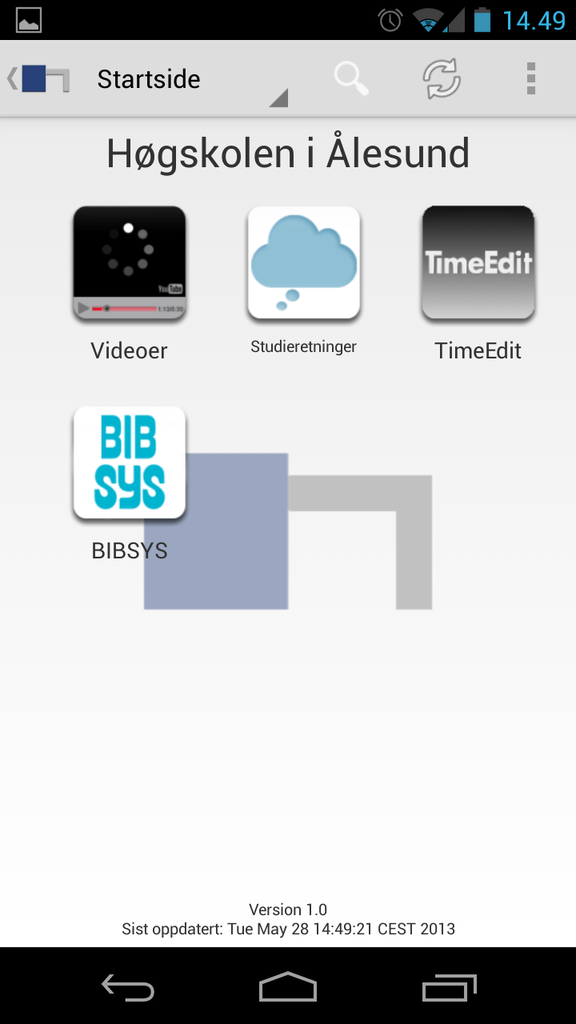
\includegraphics[width=4cm]{mobapp_timeedit.png}
                \caption{Viser TimeEdit fragmentet på fremsiden}
        \end{subfigure}
        \quad
        \begin{subfigure}[b]{0.3\textwidth}
                \centering
                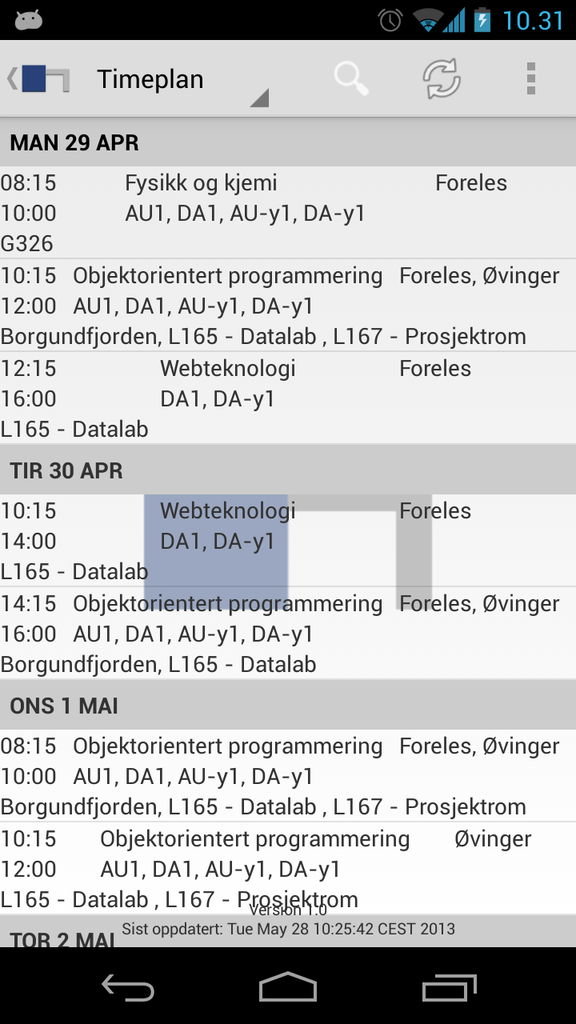
\includegraphics[width=4cm]{mobapp_timeedit2.png}
                \caption{Viser innsiden av TimeEdit fragmentet}
        \end{subfigure}
        \quad
                \begin{subfigure}[b]{0.3\textwidth}
                        \centering
                        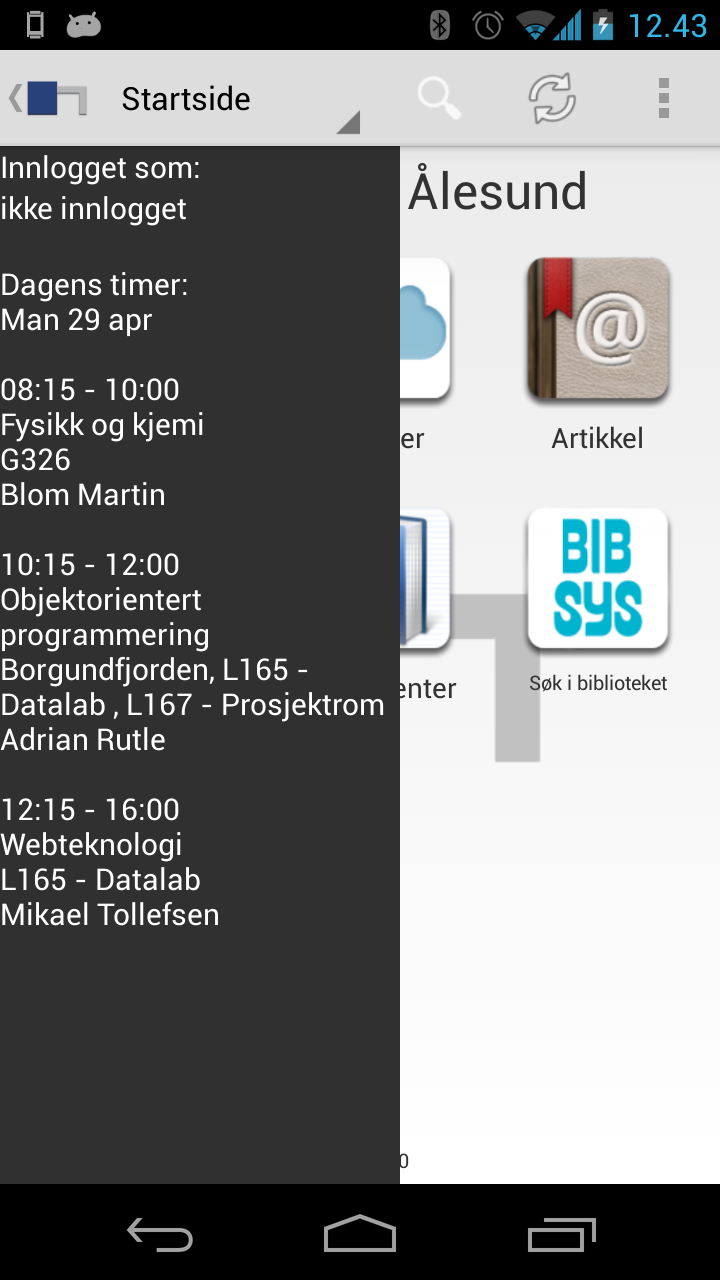
\includegraphics[width=4cm]{mobapp_timeedit3.png}
                        \caption{Viser TimeEdit i sidemenyen}
                \end{subfigure}
        \caption{Skjermbilder av TimeEdit-funksjonen til mobilapplikasjonen}
\end{figure}

TimeEdit-knappen er tilgjengelig fra hovedskjermen, og ved å trykke på den vil timeplanen for det gjeldende faget eller studiet vises fram på en lett-oversiktlig måte.
I mobilapplikasjonen er TimeEdit-funksjonalitet også tilgjengelig ved å trykke på HIALS-ikonet oppe i venstre hjørne. En meny vil gli inn fra venstre side ut som viser dagens timeplan for en satt klasse, i dette tilfellet DA1. Trykk på HIALS-ikonet igjen eller Android-tilbakeknapp nederst i venstre hjørnefor å skjule sidemenyen.








\subsection{Fronter}

\begin{figure}[H]
  \centering
  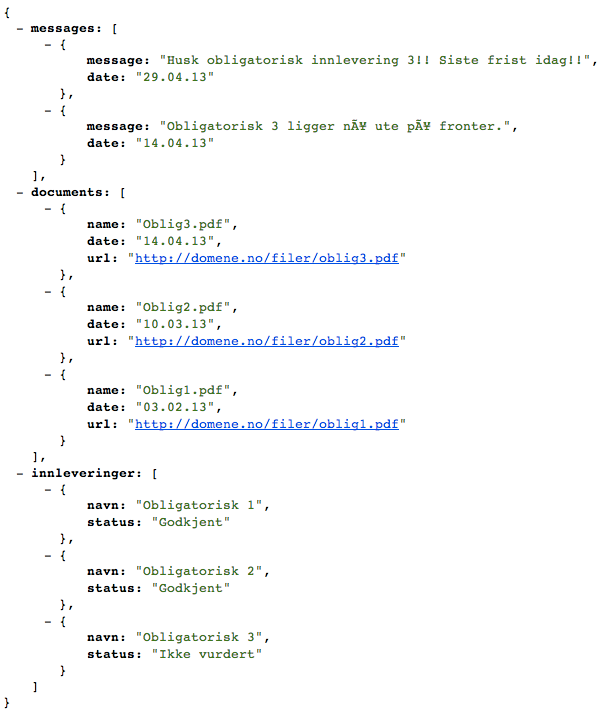
\includegraphics[width=7cm]{fronter-json.png}
  \caption{asdasdsadasdasdasdsadsads}
\end{figure}

Vi ville hente meldinger fra læreren, dokumenter og innleverings-status fra rommen på fronter.\newline
\newline
Siden vi ikke fikk den nødvendige tilgangen til skolens frontersystem valgte vi å gjøre ferdig så mye som mulig av systemet slik at det enkelt kunne tas ibruk i fremtiden når en slik tilgang foreligger. Derfor lagde vi et fast sett med eksempel-data for å vise at vår side av APIet fungerer. Det eneste som gjensto var å parse APIet til fronter.

\subsubsection{Fronter i appen}

\begin{figure}[H]
        \centering
        \begin{subfigure}[b]{0.3\textwidth}
                \centering
                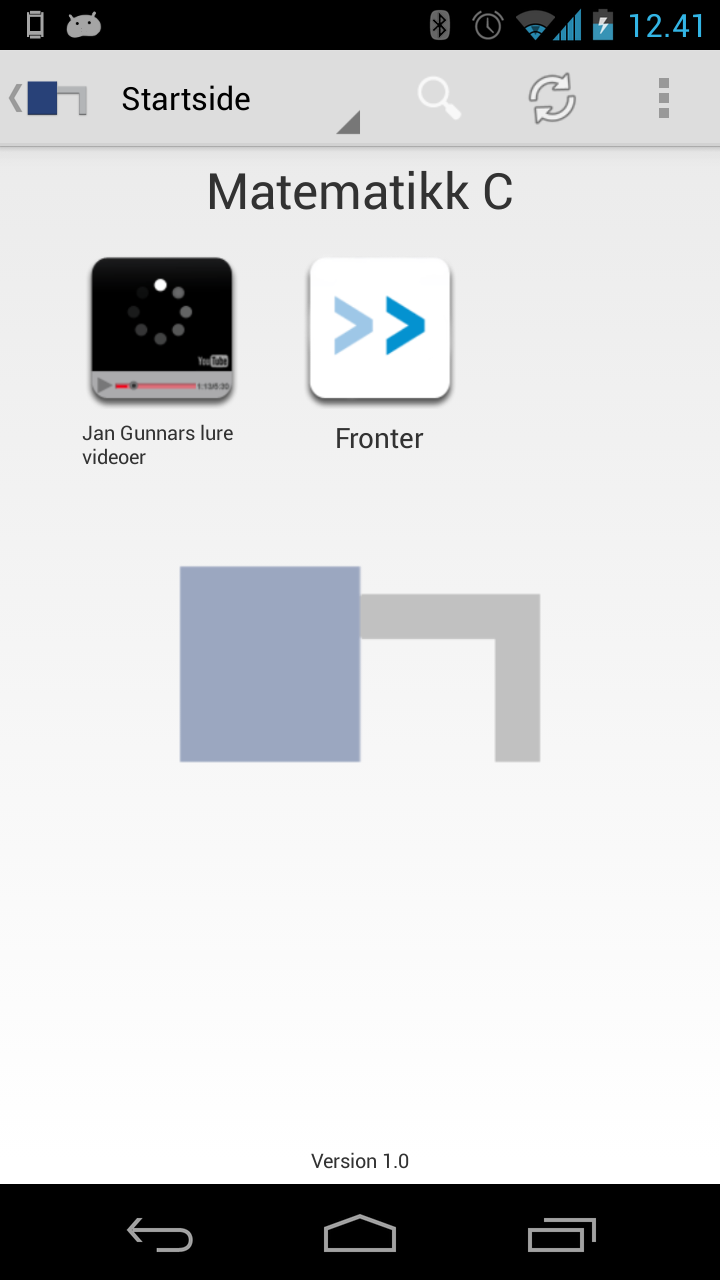
\includegraphics[width=5cm]{mobapp-fronter.png}
                \caption{Viser Fronter fragmentet på fremsiden}
        \end{subfigure}
        \quad
        \begin{subfigure}[b]{0.3\textwidth}
                \centering
                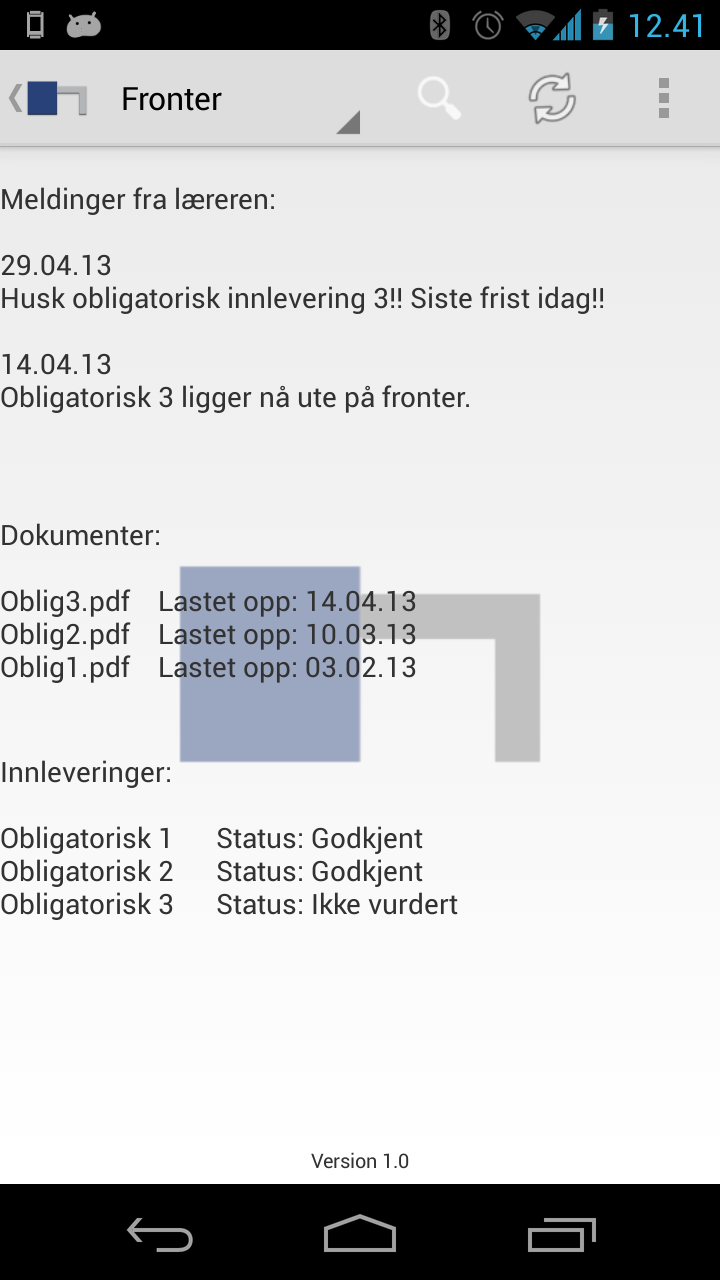
\includegraphics[width=5cm]{mobapp-fronter2.png}
                \caption{Viser innsiden av Fronter fragmentet}
        \end{subfigure}
        \caption{Skjermbilder av Fronter-funksjonen til mobilapplikasjonen}
\end{figure}

Fronter fragmentet viser informasjon fra et valgt rom på fronter og kan kun legges til på fag laget. Siden implenentasjonen ikke ble fullført vises kun eksempeldata her. Om fronter implementasjonen blir fullført i fremtiden er integrasjonen i mobilapplikasjonen allerede klar til bruk. 

\subsection{BibSys}

Det første som måtte gjøres var å definere hvilke funksjoner som skulle implementeres. De mer gjennomførte søkesidene på nettet tilbyr mange muligheter for tilpassede søkekriterier, slik som tittel, forfatter, ISBN, bibliotek, etc. \endnote{\url{http://ask.bibsys.no/ask/action/stdsearch} - 21.05.2013} Gruppen ble enige om å begrense funksjonaliteten til et enkelt søk på tittel, begrenset til beholdningen til biblioteket ved Høgskolen i Ålesund. Resultatet av dette søket skulle vises i en liste i mobilapplikasjonen.\newline
\newline
For å få tilgang til databasen til BIBSys tok vi kontakt med support på BIBSys ved hjelp av vår kontaktperson ved skolens bibliotek, Monica Marchant. Derifra ble det informert om at det grensesnittet de hadde som passet best til vårt var SRU(search/retrieve via URL). Dette er en metode hvor man setter søkeparametrene sine inn i en URL, og så svarer serveren med resultatet i form av et XML dokument.
\newline
Først måtte vi altså lage en mal til URL’en slik at vi kunne enkelt putte inn søkeparametrene vi ønsket. Ved hjelp av noen eksempler fra BIBSys sin support kom vi frem til følgende mal:
\newline
\begin{lstlisting}[language=HTML, frame=single]
http://sru.bibsys.no/search/biblio?version=1.2\&operation=searchRetrieve\&startRecord=1\&maximumRecords=10\&query=bs.bibkode=xb\%20AND\%20bs.tittel=ibsen
\end{lstlisting}
I denne url malen er det noen faste og variable parametre. Disse er som følger:

\begin{table}[H]
\begin{center}
\caption{DASDSADSADASDASDASDASDASDADASD}
  \begin{tabular}{ | p{4cm} | p{8cm} | p{2cm} |}
    \hline
    Parameter & Betydning & Fast/variabel \\ \hline
    maximumRecords=10 & Dette parametret gir at det skal ikke returneres mer enn de 10 første resultatene & Fast \\ \hline
    query=bs.bibkode=xb & Dette parametret begrenser søket til Biblioteket ved Høgskolen i Ålesund & Fast \\ \hline
    query=...bs.tittel=ibsen & Dette parametret begrenser søket til bøker med tittel som ligner på order “ibsen”. Man søker på forskjellige titler ved å forandre på tittel parametret. & Variabel \\
    \hline
  \end{tabular}
\end{center}
\end{table}

Ved å bruke denne eksempel URL’en i en nettleser vil man kunne se resultatene som blir returnert fra BibSys sine servere.\newline
\newline
Nå som vi visste hvordan man søker i BibSys sine databaser, og hva vi kunne vente oss tilbake, måtte vi avgjøre hva slags struktur systemet vårt skulle ha. Av tidligere erfaring fra alle de andre funksjonene som applikasjonen allerede tilbyr ble vi enige om at serveren skulle ta seg av spørringen til BibSys sine systemer og prossesere resultatet til et enklere format. Mobilapplikasjonen vil da kunne gjøre en enkel spørring mot serveren, og så tar serveren seg av spørringen og parsingen, og gir tilbake et enkelt resultat. På denne måten vil det også være enkelt å oppdatere løsningen i frtemtiden, da alle forandringer vil skje på serveren, og brukerne ikke trenger å oppdatere. Om det blir lagt til noen nye funksjoner, vil man alikevel måtte oppdatere mobilapplikasjonen.

\begin{figure}[H]
  \centering
  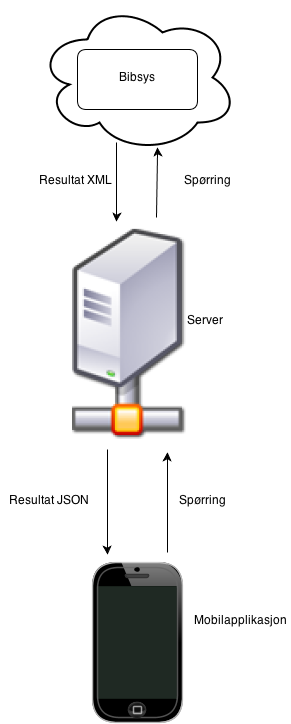
\includegraphics[width=5cm]{BibsysDiagram.png}
  \caption{asdasdsadasdasdasdsadsads}
\end{figure}

Som man kan se er det veldig mye informasjon som blir returnert, så vi måtte finne en måte å hente ut kun de dataene som var relevante. For å løse dette valgte vi å bruke Javabiblioteket Jsoup som vi allerede hadde brukt tidligere for å hente ut data fra timeplansystemet TimeEdit. Dette var fordi biblioteket hadde vist seg å være ypperlig til å hente ut data fra store og kompliserte datasett.\newline
\newline
For å hente ut de relevante dataene, søkte vi igjennom xml filen, og hentet ut infoen som ligger ved tag id 245. Denne under-seksjonen inneholder navnet på forfatter, tittel, og undertittel.
\begin{figure}[H]
  \centering
  \includegraphics[width=10cm]{bibsysstuff.png}
  \caption{asdasdsadasdasdasdsadsads}
\end{figure}

Her går koden igjennom seksjonen linje for linje, og skreller vekk alt som ikke skal være med. Til slutt lagres tittelen og forfatternavnet i en enkel entityklasse og settes inn i listen som skal returneres til mobilapplikasjonen.\newline
\newline
Man kan se tydelig hvordan jobben serveren gjør forenkler jobben for mobilapplikasjonen. Dataene serveren mottar fra BibSys er på venstre side, mens dataene serveren sender videre til mobilapplikasjonen etter å ha parset innholdet står på høyre. XML dokumentet har forøvrig blitt kortet ned med ca. 2/3 av plasshensyn.

\begin{figure}[H]
  \centering
  \includegraphics[width=14cm]{XML-JSON-Comparison.png}
  \caption{asdasdsadasdasdasdsadsads}
\end{figure}

BibSys APIet i webapplikasjonen er tilgjengelig via URLen: domene.no/services/bibsys/<søkestreng> der <søkestreng> er hva som spurt om i BibSys sitt eget API.

\subsubsection{BibSys i appen}

\begin{figure}[H]
  \centering
  \includegraphics[width=7cm]{mobapp-bibsys.png}
  \caption{Skjermbilde fra mobilapplikasjonen - Her vises resultatet etter et søk på bøker som matchet tittelen “ibsen}
\end{figure}

I mobilapplikasjonen er BibSys implementert som et fragmentet og kan kun settes inn på fremsiden som er det øverste laget. I fragmentet er det en tekstboks og en knapp, brukeren skriver inn søkestrengen og trykker på knappen. Når knappen trykkes inn sendes en spørring med søkestrengen til BibSys API’et i webapplikasjonen. JSON dataen fra REST tjenesten blir hentet og parset av mobilapplikasjonen og vist i skjermbildet.

\newpage

\end{document}